\section{Applications of Generating Functions}
\begin{exercise}
    Given a coin whose probability of turning up `heads' is $p$, let $p_n$ be the probability that the first occurrence of `heads' is at the $n$th toss of the coin. Evaluate $p_n$ and the opsgf of the sequence $\{p_n\}$. Use that opsgf to find the mean of the number of trials till the first `heads' and the standard deviation of that number.
\end{exercise}
\begin{solution}
    Clearly, $p_n = (1-p)^{n-1}p$ ($n-1$ times tails and then heads) with opsgf:
    \[
        P(x) = \sum_{n= 1}^\infty p_n x^n= \sum_{n=1}^\infty (1-p)^{n-1}p x^n = px \bsum (1-p)^n x^n \estep{\eqref{eq:power_geom}} \frac{px}{1-(1-p)x}
    \]
    The mean number of trials is given by 
    \[\mu = P'(1) = \left\{\frac{p(1-(1-p)x) + (1-p)px}{(1-(1-p)x)^2}\right\}_{x=1} = \frac{1}{p}\] and the variance by:
    \begin{align*}
        \sigma^2 &= \{(\log P)' + (\log P)''\}_{x=1} \\
        &= \left\{\frac{1}{px^2-x^2 + x} + \frac{-2(p-1)x-1}{x^2((p-1)x+1)^2}\right\}_{x=1} \\
        &= \frac{1-p}{p^2}
    \end{align*}
\end{solution}

\begin{exercise}
    In the \emph{coupon collector's problem} we imagine that we would like to get a complete collection of photos of movie stars, where each time we buy a box of cereal we acquire one such photo, which may of course duplicate one that is already in our collection. Suppose there are $d$ different photos in a complete collection. Let $p_n$ be the probability that exactly $n$ trials are needed in order, for the first time, to have a complete collection.
    \begin{enumerate}[label=(\alph*)]
        \item Show that
        \[
            p_n = \frac{d!\stirlingSnd{n-1}{d-1}}{d^n},
        \]
        where $\stirlingSnd{n}{k}$ is the Stirling number of the second kind.
        \item Let $p(x) \stackrel{ops}{\longleftrightarrow} \{p_n\}$. Show that 
        \[
            p(x) = \frac{(d-1)!x^d}{(d-x)(d-2x)\cdots(d-(d-1)x)}
        \]
        \item Find, directly from the generating function $p(x)$, the average number of trials that are needed to get a complete collection of all $d$ coupons.
        \item Similarly, using $p(x)$, find the standard deviation of that number of trials.
        \item In the case $d=10$, how many boxes of cereal would you expect to have to buy in order to collect all $10$ different kinds of pictures.
    \end{enumerate}
\end{exercise}
\begin{solution}
    \begin{enumerate}[label=(\alph*)]
        \item Consider a sequence of $n$ photos such that the $n$th photo completes the collection. Take the first $n-1$ photos and construct an ordered partition of $n-1$ in $d-1$ classes the following way: if the $i$th type of photo was chosen (with $1\leq i \leq d)$ as the $j$th photo, then put $j$ in the $i$th class. Note that there are now $d-1$ nonempty classes (it cannot be $d$ or the collection would have been complete and it cannot be less than $d-1$ or the collection would be impossible to complete with one more photo).
        
        Note that this process is also reversible from an ordered partition of $n-1$ elements into $d-1$ nonempty classes where one class is empty. Since there are $\stirlingSnd{n-1}{d-1}$ of unordered partitions, there are $(d-1)!\stirlingSnd{n-1}{d-1}$ ordered partitions. Since there are $d$ choices for the last photo and there are $d^n$ possible sequences in total, we find:
        \[
            p_n = \frac{d!\stirlingSnd{n-1}{d-1}}{d^n}
        \]
        \item 
        \[
            p(x) = \bsum[n] p_n x^n = \sum_{n=1}^\infty d! \stirlingSnd{n-1}{d-1}\left(\frac{x}{d}\right)^n = (d-1)! x \bsum[n] \stirlingSnd{n}{d-1} \left(\frac{x}{d}\right)^{n}
        \]
        Use \eqref{eq:stSnd} to obtain the result:
        \begin{align*}
            p(x) \estepalign{\eqref{eq:stSnd}} (d-1)!x \frac{\frac{x^{d-1}}{d^{d-1}}}{\left(1-\frac{x}{d}\right)\left(1-2\frac{x}{d}\right)\cdots \left(1-(d-1)\frac{x}{d}\right)} \\
            &= \frac{(d-1)!x^d}{(d-x)(d-2x)\cdots (d-(d-1)x)}
        \end{align*}
        \item \hypertarget{eq:ch4:2:c}{} The average number of trials is:
        \[
            \mu = p'(1) = \frac{d!(d-1)! - (d-1)! \sum_{i=1}^{d-1} -i\frac{(d-1)!}{d-i}}{(d-1)!^2}
        \]
        Dividing through and reversing the summation:
        \[
            \mu = d + \sum_{j=1}^{d-1} \frac{d-j}{j} = 1 + \sum_{j=1}^{d-1}\frac{d}{j} = d\sum_{j=1}^{d} \frac{1}{j}
        \]
        \item \hypertarget{eq:ch4:2:d}{} The variance is given by:
        \[
            \sigma^2 = \{(\log p(x))' + (\log p(x))''\}_{x=1} = d + \sum_{i=1}^{d-1} \frac{i}{d-i} - d + \sum_{i=1}^{d-1} \frac{i^2}{(d-i)^2}
        \]
        Reversing the summations and doing some algebraic manipulations:
        \begin{align*}
           \sigma^2 &= \sum_{j=1}^{d-1} \frac{d-j}{j} + \sum_{j=1}^{d-1} \frac{(d-j)^2}{j^2} \\
            &= -(d-1) + (d-1) + \sum_{j=1}^{d-1} \left(\frac{d}{j} + \frac{d^2}{j^2} -2 \frac{d}{j}\right) \\
            &= d\sum_{j=1}^{d-1} \left(\frac{d}{j^2} - \frac{1}{j}\right)
        \end{align*}
        \item From part \hyperlink{eq:ch4:2:c}{(c)} and \hyperlink{eq:ch4:2:d}{(d)}, we find
        \[
            \mu = 10\sum_{j=1}^{10} \frac{1}{j} = 29.3, \qquad \sigma^2 = 10 \sum_{j=1}^{9} \frac{10}{j^2} - \frac{1}{j} = 125.7
        \]
    \end{enumerate}
\end{solution}

\begin{exercise}
    (First return time on trees) By a \emph{random walk} on a graph we mean a walk among the vertices of the graph, which, having arrived at some vertex $v$, goes next to a vertex $w$ that is chosen uniformly among the neighbors of $v$ in the graph.

    If $T$ is a tree, and $v$ is a vertex of $T$, let $p(j;v;T)$ denote the probability that a random walk on $T$ which starts at vertex $v$, returns to $v$ for the first time after exactly $j$ steps.

    Now let $T_1$, $T_2$ be trees, let $v_i$ be a vertex of $T_i$ for $i=1,2$, and let $T$ be the tree that is formed from these two by adding edge $(v_1, v_2)$. Finally, let $F_1(x;v_1)$, $ F_2(x;v_2)$, $F(x;v_1)$ be the opsgf's of the sequences $\{p(j;v_1;T_1)\}_{j\geq0}$, $\{p(j;v_2;T_2)\}_{j\geq0}$, and $\{p(j;v_1;T)\}_{j\geq0}$, respectively.
    \begin{enumerate}[label=(\alph*)]
        \item Show that 
        \[
            F(x;v_1) = \frac{1}{d_1+1}\left\{d_1F_1(x;v_1) + \frac{x^2}{d_2+1-d_2F_2(x;v_2)}\right\}
        \]
        where $d_i$ is the degree of the vertex $v_i$ in the tree $T_i$, for $i=1,2$.
        \item Let $\mu_T(a)$ be the \emph{average} number of steps in a random walk that starts at vertex $a\in T$ and stops when it returns to $a$ for the first time. Show, by differentiating the answer to part (a), that
        \[
            \mu_T(v_1) = \frac{1}{d_1+1}(2+d_1\mu_{T_1}(v_1) + d_2\mu_T(v_2))
        \]
        \item Let the tree $T$ be a path of $n+1$ vertices. Show that the mean return time of a walk that begins at vertex $v$ is $2n$ if $v$ is one of the two endpoints, and is $n$ for all other $v$ (surprisingly?).
        \item Again, if $T$ is a path of $n$ vertices and if $P_n(x)$ denotes the generating function $F(x;v_1)$ of part (a), where $v_1$ is an endpoint of $T$, then find an explicit formula for $P_n(t)$.
    \end{enumerate}
\end{exercise}
\begin{solution}
    \begin{enumerate}[label=(\alph*)]
        \item \hypertarget{eq:ch4:3:a}{} Starting from $v_1$, its first step is either into $T_1$ or $T_2$ (via $v_2$). In the first case, the probability is:
        \[
            \frac{d_1}{d_1+1} p(j;v_1;T_1)
        \]
        where the first term is the probability of choosing a step into $T_1$ and the second term is the first return probability starting from $v_1$ in $T_1$ with $j$ steps.

        The second case is more difficult since $v_2$ may be hit multiple times before returning to $v_1$, so $p(j-2,v_2,T_2)$ cannot be trivially used. Let $m$ be the times $v_2$ gets hit which are not fixed (so not the first and last time). Then the contributed probability is:
        \[
            \frac{1}{1+d_1}\frac{1}{1+d_2}\sum_{j_1+\ldots + j_m = j-2} \frac{d_2}{1+d_2}p(j_1;v_2;T_2)\cdots \frac{d_2}{1+d_2}p(j_m;v_2;T_2)
        \]
        The first coefficients comes from the first step from $v_1$ to $v_2$. The second coefficients accounts for the last step back from $v_2$ to $v_1$. Then the summand contains $m$ terms which denote walks in $T_2$ of length $j_i$ starting at $v_2$ and ending in $v_2$ (without hitting $v_2$ in between). The sum iterates over all possible combination of intermediate path lengths. Now note that this probability can also be written as (following the rules of multiplication of opsgf's):
        \[
            \frac{1}{1+d_1}\frac{1}{1+d_2}\left(\frac{d_2}{1+d_2}\right)^m \coeff{x^{j-2}} F_2(x;v_2)^m
        \]
        Summing over all possible $m$ values gives:
        \[
            \frac{(1+d_1)^{-1}}{1+d_2}\coeff{x^{j-2}}\bsum[m] \left(\frac{d_2F_2(x;v_2)}{1+d_2}\right)^m \estep{\eqref{eq:power_geom}} \coeff{x^{j-2}} \frac{(1+d_1)^{-1}}{1+d_2-d_2F_2(x;v_2)}
        \]
        Combining this result with the first case, multiplying by $x^j$ and summing over $j$ gives the required result:
        \begin{align*}
            F(x;v_1) &= \bsum[j] p(j;v_1;T)x^j \\
            &= \bsum[j] \frac{d_1p(j;v_1;T_1)x^j}{d_1+1} + x^j\coeff{x^{j-2}}\frac{1}{(d_1+1)(1+d_2-d_2F_2(x;v_2))} \\
            &= \frac{1}{d_1+1}\left\{d_1F_1(x;v_1) + \frac{x^2}{1+d_2-d_2F_2(x;v_2)}\right\}
        \end{align*}
        \item \hypertarget{eq:ch4:3:b}{} Noting that:
        \[
            \mu_{T_i}(v_i) = \frac{F_i'(1;v_i)}{F_i(1;v_i)} = F_i'(1;v_i)
        \]
        for $i=1,2$ since the $F_i$ encode probability distributions and therefore sum to~$1$, we immediately find:
        \begin{align*}
            \mu_T(v_1) &= \frac{1}{d_1+1} \left(d_1F_1'(1;v_1) + \frac{2(1+d_2-d_2F_2(1;v_2)) + d_2F_2'(1;v_2)}{(1+d_2-d_2F_2(1;v_2))^2} \right) \\
            &= \frac{1}{d_1+1}  \left(d_1\mu_{T_1}(v_1) + \frac{2(1+d_2-d_2) +d_2\mu_{T_2}(v_2)}{(1+d_2-d_2)^2}\right) \\
            &= \frac{1}{d_1+1}(2+d_1\mu_{T_1}(v_1) + d_2\mu_{T_2}(v_2))
        \end{align*}
        \item The result is clearly true for $n=0$ (one vertex: the mean return time is~$0$) and $n=1$ (two vertices which are both endpoints: the mean return time is $2$).
        
        We proceed by induction. Assume the mean return for the endpoints in a path of $n+1$ vertices is $2n$ for $n\leq 1$, we show that the statement also holds for $n+2$ vertices. Let $v$ be an endpoint in a path $T$ with $n+2$ vertices. Now split the path into two pieces: a path $T_1$ of size $1$ containing only $v$ and a path $T_2$ of size $n+1$ containing the other vertices. Assume that the vertex which was connected to $v$ is called $w$. We now use the formula from part \hyperlink{eq:ch4:3:b}{(b)} with $\mu_{T_1}(v) = 0$ and $\mu_{T_2}(w) = 2n$ per the induction hypothesis:
        \[
            \mu_T(v) = \frac{1}{1+0} (2 + 0\cdot 0 + 1\cdot2n) = 2(n+1)
        \]
        Note that $d_1= 0$ because it is a single vertex and $d_2=1$ since it is an endpoint (it at least has one neighbour since we assume $n+1 \geq 2$). Due to the principle of induction, the hypothesis is true for all $n$.  

        Now, let $v$ be a vertex which is not an endpoint. As an additional edge case, we see that for $n=2$ (three vertices), the midpoint indeed has mean return time $2$ (since there are only two possible walks, both of size $2$).

        Knowing that the mean return time for $n + 1$ vertices is $2n$, let $v$ be a vertex which is not an endpoint in a path $T$ with $n+1$ vertices (where $n\geq 3$). Now break the path into two paths such that both paths contain more than $2$ vertices and $v$ is an endpoint of one path (this split is always possible for $n\geq 3$). Let $w$ be the vertex which was connected to $v$ and call the sizes of both paths $i$ and $j$ such that $i+j=n+1$. Now, from part (b), we have:
        \[
            \mu_T(v) = \frac{1}{1+1}(2+1\cdot 2(i-1) + 1\cdot2(j-1)) = n
        \]
        since the degree of both $v$ and $w$ are $1$ and they are both endpoints in their respective path.
        \item Since $v_1$ is an endpoint of $T$, we can again split the path into two paths where one only contains the vertex $v_1$ and the other part contains the remaining $n-1$ vertices. We then have by part \hyperlink{eq:ch4:3:a}{(a)} that:
        \[
            P_n(x) = \frac{1}{0+1} \left\{0\cdot P_1(x;v_1) + \frac{x^2}{1+1-1\cdot P_{n-1}(x)}\right\} = \frac{x^2}{2-P_{n-1}(x)}
        \]
        for $n\geq2$. Since $P_1(x)=1$, the form of the recurrence suggests that $P_n(x)$ will be a rational function in $x$. Therefore, let $P_n(x) = \frac{A_n(x)}{B_n(x)}$. Then we have:
        \[
            \frac{A_n(x)}{B_n(x)} = \frac{x^2B_{n-1}(x)}{2B_{n-1}(x) - A_{n-1}(x)}
        \]
        which is satisfied if
        \[
            \begin{cases}
                A_n = x^2B_{n-1} \\
                B_n = 2B_{n-1} -x^2B_{n-2}
            \end{cases}
        \]
        We first solve the difference equation for $B_n(x)$. Assume $B_n(x) = b(x)^n$ gives:
        \[
            b(x)^{n} = 2b(x)^{n-1}-x^2b(x)^{n-2}
        \]
        from which we find
        \[
            b(x)^2 - 2b(x) - x^2 = 0 \Longleftrightarrow b(x) = 1\pm \sqrt{1-x^2}
        \]
        and
        \[
            B_n(x) = c_0 \left(1+\sqrt{1-x^2}\right)^n + c_1\left(1-\sqrt{1-x^2}\right)^n = c_0b_+^n + c_1 b_-^n
        \]
        where $b_{\pm} = 1\pm\sqrt{1-x^2}$ respectively. Take as initial condition $B_1 = B_2 = 1$ to satisfy $P_1=1$ and $P_2=x^2$, resulting in:
        \[
            \begin{cases}
                c_0b_+ + c_1b_- = 1 \\
                c_0b_+^2 + c_1b_-^2 =1
            \end{cases} \implies  \begin{cases}
                c_0 = \frac{1}{2b_+} \\
                c_1 = \frac{1}{2b_-}
            \end{cases}
        \]
        leading to the end result:
        \[
            P_n(x) = \frac{A_n(x)}{B_n(x)} =  \frac{x^2B_{n-1}(x)}{B_n(x)} =  x^2 \left(\frac{b_+^{n-2} + b_-^{n-2}}{b_+^{n-1} + b_-^{n-1}}\right) 
        \]
    \end{enumerate}
\end{solution}

\begin{exercise}
    Find, in terms of $N(x)$, the opsgf of the sequences $\{e_{\leq m}\}$ (respectively, $\{e_{\geq m}\}$) which count the objects that have \emph{at most $m$} properties (respectively, at least $m$ properties).
\end{exercise}
\begin{solution}
    The sequence $\{e_{\leq m}\}$ is equivalent to the partial sum sequence of $\{e_m\}$. We therefore have:
    \[
        \bsum[m] e_{\leq m}x^m = \frac{E(x)}{1-x} \estep{\eqref{eq:sieve}} \frac{N(x-1)}{1-x}
    \]
    Observe that the total number of objects is $N(0)$ because:
    \[
        N(0) = N_0 = \sum_{|S| = 0} N(\supseteq S) = N(\supseteq \emptyset) = N
    \]
    such that $e_{\geq m} = N(0) - e_{\leq m-1}$ with opsgf:
    \[
        \bsum[m] e_{\geq m}x^m =  \bsum[m] (N(0) - e_{\leq m-1})x^m = \frac{N(0)}{1-x} - \frac{xN(x-1)}{1-x}
    \]
\end{solution}

\begin{exercise}
    What chessboard would you use to derive the number of permutations that have no fixed points? Rederive the formula for this number using the chessboard method.
\end{exercise}
\begin{solution}
    Choose a chessboard containing only the diagonal cells $(i, i)$ for $1\leq i \leq n$, then $r_k = \binom{n}{k}$ since any selection of $k$ distinct cells is valid to place $k$ nonattacking rooks. We then have:
    \[
        N(x) = \bsum[k] (n-k)!\binom{n}{k}x^k 
    \]
    Now, the number of permutations with no fixed points corresponds to the constant coefficient of $E(x)$ since the permutation is not permitted to meet the chessboard in any square (or it would mean that $(i, \sigma(i)) = (i, i) \in C$ which is a fixed point). We find:
    \[
        e_0 = \coeff{x^0}\sum_{k=0}^n (n-k)! \frac{n!}{k!(n-k)!}(x-1)^k = n! \sum_{k=0}^n \frac{(-1)^k}{k!}
    \]
    which indeed corresponds to the number of permutations with no fixed points.
\end{solution}

\begin{exercise}
    \label{ex:4:6}
    (Bonferroni's inequalities) In the sieve method, 
    \[
        e_0 = E(0) = N(-1) = \sum_t (-1)^tN_t
    \]
    computes the number of objects that have no properties at all. Suppose the alternating series on the right were cut off after a certain value $t=m$, say. Show that the result would overestimate $e_0$ if $m$ were even and underestimate it for $m$ odd.

    To do this, show that the sequence
    \[
        \alpha_m =\sum_{r\geq m}(-1)^{r-m}N_r \quad (m=0,1,2,\ldots)
    \]
    has the opsgf $e_0 + x\sum_{r\geq 0} e_{r+1}(x+1)^r$, whose coefficients are obviously nonnegative.
\end{exercise}
\begin{solution}
    Finding the opsgf for $\alpha_m$:
    \[
        \bsum[m]\alpha_mx^m = \bsum[m] \sum_{r=m}^\infty (-1)^{r-m}N_r x^m
    \]
    The domain of summation is:
    \[
        \includegraphics[width=0.5\textwidth]{supplements/ch4/ex4_6.pdf}
    \]
    Swapping the summations therefore gives:
    \[
        \bsum[m] \alpha_mx^m = \bsum[r] \sum_{m=0}^r (-1)^{r-m}N_r x^m = \bsum[r] (-1)^r N_r \sum_{m=0}^r (-x)^m
    \]
    Evaluating the geometric sum:
    \begin{align*}
        \bsum[m] \alpha_mx^m &= \bsum[r] (-1)^r N_r \frac{1-(-x)^{r+1}}{1+x} \\
        &= \frac{1}{1+x} \bsum[r] (-1)^rN_r - (-1)^{2r+1} N_r x^{r+1} \\
        &= \frac{1}{1+x} \bsum[r](-1)^rN_r  +N_rx^{r+1}
    \end{align*}
    Note that summing the first term in the summation is just $N(-1) = E(0) = e_0$:
    \[
        \bsum[m] \alpha_mx^m = \frac{1}{1+x} \left(e_0 + \bsum[r] N_rx^{r+1}\right) = \frac{e_0 + x\bsum[r]N_rx^r}{1+x} = \frac{e_0 + xN(x)}{1+x}
    \]
    Using the relation between $N(x)$ and $E(x)$ \eqref{eq:sieve}
    \[
        \bsum[m] \alpha_mx^m = \frac{e_0 + xE(x+1)}{1+x}
    \]
    Expanding $E(x+1)$ in its power series:
    \[
        \bsum[m] \alpha_mx^m = \frac{e_0 + x\left( e_0 + e_1(x+1) + \cdots \right)}{1+x} = e_0 + x \bsum[r] e_{r+1}(x+1)^r
    \]
    Since the coefficients are obviously nonnegative, we have that $\alpha_m \geq 0$ and therefore the truncated alternating series overestimates $e_0$ if $m$ is even and underestimates if $m$ is odd.
\end{solution}

\begin{exercise}
    (Bonferroni's inequalities, continued) Not only is $e_0$ alternately under- and overestimated by the successive partial sums of its sieve formula, the same is true of every $e_k$, the number of objects that have exactly $k$ properties. To show this generatingfunctionologically, define, for each $k,t \geq 0$,
    \[
        \gamma(k,t) = (-1)^{t+1}\left\{e_k - \sum_{j\leq t}(-1)^j \binom{k+j}{j} N_{k+j}\right\}
    \]
    Then the problem is to show that all $\gamma(k,t)\geq 0$.

    To do this,
    \begin{enumerate}[label=(\alph*)]
        \item Let $\Gamma(x,y)$ be the $2$-variable opsgf of the $\gamma$. Then multiply the definition of the $\gamma$'s by $x^ky^t$, sum over $k,t\geq 0$, and show that
        \[
            \Gamma(x,y) = \frac{E(x+(1+y))-E(x)}{(1+y)}
        \]
        \item It now follows that the $\gamma$'s are nonnegative, and in fact that 
        \[
            \gamma(k,t) = \sum_{r > k}\binom{r}{k}\binom{r-k-1}{t}e_r \qquad (k,t\geq 0)
        \]
    \end{enumerate}
\end{exercise}
\begin{solution}
    \begin{enumerate}[label=(\alph*)]
        \item Finding the opsgf of $\gamma$:
        \begin{align*}
            \sum_{k,t\geq 0} \gamma(k,t)x^k y^t = \bsum[k] \bsum[t] x^ky^t (-1)^{t+1}\left\{e_k - \sum_{j=0}^t(-1)^j \binom{k+j}{j} N_{k+j}\right\}
        \end{align*}
        Recall that:
        \[
            e_k = \bsum[t] (-1)^{t-k} \binom{t}{k}N_t
        \]
        Change of variables $j=t-k$ results in:
        \begin{equation} \label{eq:ek_alt}
            e_k = \bsum[j] (-1)^{j} \binom{k+j}{k}N_{k+j} \estep{\eqref{eq:bin_sym}}  \bsum[j] (-1)^{j} \binom{k+j}{j}N_{k+j}
        \end{equation}
        so that the opsgf for $\gamma$ can be simplified as follows:
        \begin{align*}
            \Gamma(x,y) &= \bsum[k]\bsum[t] x^k y^t (-1)^{t+1} \left\{\sum_{j = t+1}^\infty (-1)^j \binom{k+j}{j} N_{k+j}\right\} \\
            &=\bsum[k]\bsum[t] \sum_{j = t+1}^\infty x^ky^t(-1)^{t+j+1} \binom{k+j}{j} N_{k+j}
        \end{align*}
        Switching the last two summations yields:
        \begin{align*}
            \Gamma(x,y) &= \bsum[k] x^k \sum_{j=1}^\infty (-1)^{j+1}\binom{k+j}{j}N_{k+j} \sum_{t=0}^{j-1} (-y)^t \\
            &= \bsum[k] x^k \sum_{j=1}^\infty (-1)^{j+1}\binom{k+j}{j}N_{k+j} \frac{1-(-y)^j}{1+y}
        \end{align*}
        Include $j=0$ for the second summation. This is valid since the included term is $0$ anyway:
        \[
            \Gamma(x,y) = \bsum[k] x^k \bsum[j] (-1)^{j+1}\binom{k+j}{j}N_{k+j} \frac{1-(-y)^j}{1+y}
        \]
        Note that:
        \[
            \Gamma(x, y) = \frac{A(x) + B(x,y)}{1+y}
        \]
        where
        \begin{align*}
            A(x) &= \bsum[k] x^k \bsum[j](-1)^{j+1}\binom{k+j}{j}N_{k+j}  \\
            B(x, y) &= \bsum[k] x^k \bsum[j]\binom{k+j}{j}N_{k+j}y^j
        \end{align*}
        For the first sum, we recognize $e_k$ inside (see \eqref{eq:ek_alt}):
        \[
            A(x) = \bsum[k] x^k \bsum[j] (-1)^{j+1}\binom{k+j}{j}N_{k+j} = -\bsum[k]x^k e_k = -E(x)
        \]
        For the second sum, we use the binomial theorem
        \begin{align*}
            B(x,y) &=  \bsum[k]\bsum[j] \binom{k+j}{j}N_{k+j}x^ky^j \\
            &= \bsum \left\{ \sum_{j=0}^{n} x^{n-j}y^j\binom{n}{j} \right\} N_n \\
            \estepalign{\eqref{eq:binom_num2}} \bsum (x+y)^n N_n
        \end{align*}
        This is equivalent to $N(x)$ formally substituted with $x+y$ for $x$:
        \[
            B(x,y) = N(x+y)
        \]
        From the relation between $N(x)$ and $E(x)$ \eqref{eq:sieve}:
        \[
            B(x,y) = E(x+y+1)
        \]
        Combining these two sums, the required result is found:
        \[
            \Gamma(x,y) = \frac{E(x+y+1) - E(x)}{1+y}
        \]
        \item Extracting the coefficient of $x^ky^t$:
        \[
            \gamma(k,t)= \coeff{x^ky^t}\frac{E(x+y+1) - E(x)}{1+y} = \coeff{x^ky^t} \left\{\frac{E(x+y+1)}{1+y} - \frac{E(x)}{1+y}\right\}
        \]
        The desired coefficient from the first term is:
        \[
            \coeff{x^ky^t}\frac{E(x+y+1)}{1+y} = \coeff{x^ky^t} \bsum[r] e_r \frac{(x+(1+y))^r}{1+y}
        \]
        Applying the binomial theorem twice:
        \begin{align*}
            \coeff{x^ky^t}\frac{E(x+y+1)}{1+y} \estepalign{\eqref{eq:binom_num2}} \coeff{x^ky^t} \bsum[r] \infsum[l] e_rx^l (1+y)^{r-l-1} \binom{r}{l} \\
            \estepalign{\eqref{eq:binom_num}}  \coeff{x^ky^t} \bsum[r] \infsum[l] \infsum[s] e_rx^l y^s \binom{r-l-1}{s} \binom{r}{l} \\
            &=  \bsum[r] e_r \binom{r-k-1}{t} \binom{r}{k} \\
            &= \sum_{r=k}^\infty e_r \binom{r-k-1}{t} \binom{r}{k}
        \end{align*}
        Splitting off the first term from the summation
        \[
            \coeff{x^ky^t}\frac{E(x+y+1)}{1+y} = e_k \binom{-1}{t} \binom{r}{0} + \sum_{r=k+1}^\infty e_r \binom{r-k-1}{t} \binom{r}{k}
        \]
        Because $\binom{-1}{t} = \frac{(-1)(-2)\cdots (-t)}{t!} = (-1)^t$:
        \[
            \coeff{x^ky^t}\frac{E(x+y+1)}{1+y} = e_k (-1)^t + \sum_{r=k+1}^\infty e_r \binom{r-k-1}{t} \binom{r}{k}
        \]
        The desired coefficient from the second term is:
        \[
            \coeff{x^ky^t}\frac{E(x)}{1+y} \estep{\eqref{eq:power_geom}} \coeff{x^ky^t} \bsum (-1)^ny^n \bsum[m] e_m x^m = (-1)^t e_k
        \]
        Combining these two terms gives:
        \begin{align*}
            \gamma(k,t) &= \coeff{x^ky^t}\frac{E(x+y+1)}{1+y} - \coeff{x^ky^t}\frac{E(x)}{1+y} \\
            &= e_k (-1)^t + \sum_{r=k+1}^\infty e_r \binom{r-k-1}{t} \binom{r}{k} - (-1)^t e_k \\
            &= \sum_{r=k+1}^\infty e_r \binom{r-k-1}{t} \binom{r}{k}
        \end{align*}
    \end{enumerate}
\end{solution}

\begin{exercise}
    Show that 
    \[
        \sum_r \binom{n}{\left\lfloor \frac{r}{2} \right\rfloor}x^r = (1+x)(1+x^2)^n 
    \]
    Then use Snake Oil to evaluate
    \[
        \sum_k \binom{n}{k} \binom{n-k}{\left\lfloor\frac{m-k}{2}\right\rfloor}y^k
    \]
    explicitly, when $y=\pm 2$ (due to  D.\ E.\ Knuth). Find the generating function of these sums, whatever the value of $y$.
\end{exercise}
\begin{solution}
    Writing out the sum:
    \begin{align*}
        \bsum[r] \binom{n}{\left\lfloor \frac{r}{2} \right\rfloor}x^r &= 1 + x + \binom{n}{1}(x^2 + x^3) + \binom{n}{2}(x^4 + x^5) + \ldots \\
        &= (1+x) \left(1 + \binom{n}{1}x^2 + \binom{n}{2}x^4 + \ldots\right) \\
        &= (1+x) \bsum[k] \binom{n}{k}x^{2k} \\
        \estepalign{\eqref{eq:binom_num}} (1+x)(1+x^2)^n
    \end{align*}
    Let $f(m)$ denote the sum to be evaluated; multiplying by $x^m$ and summing over $m$ gives:
    \[
        F_n(x,y) = \bsum[m] \bsum[k] \binom{n}{k} \binom{n-k}{\left\lfloor\frac{m-k}{2}\right\rfloor}y^k x^m = \bsum[k] \binom{n}{k}y^k \bsum[m] \binom{n-k}{\left\lfloor\frac{m-k}{2}\right\rfloor}x^m
    \]
    Multiplying by $x^kx^{-k}$ to match the coefficient of $m-k$:
    \[
        F_n(x,y) = \bsum[k] \binom{n}{k}y^kx^k \bsum[m] \binom{n-k}{\left\lfloor\frac{m-k}{2}\right\rfloor}x^{m-k}
    \]
    Applying the above identity:
    \[
        F_n(x,y) = \bsum[k] \binom{n}{k}(xy)^k (1+x)(1+x^2)^{n-k}
    \]
    Applying the binomial theorem:
    \[
        F_n(x,y) = (1+x)(xy + 1 + x^2)^n
    \]
    For $y= 2$, we find:
    \[
        F_n(x) = (1+x)(1+ 2x+x^2)^n= (1+x)(1+ x)^{2n} = (1+x)^{2n+1}
    \]
    Extracting the $m$th coefficient:
    \[
        f(m) = \coeff{x^m}(1+x)^{2n+1} = \binom{2n+1}{m}
    \]
    For $y=-2$, we find:
    \[
        F_n(x) = (1+x)(1- 2x+x^2)^n = (1+x)(1- x)^{2n} 
    \]
    Extracting the $m$th coefficient gives:
    \[
        f(m) = \coeff{x^m} (1+x) \bsum[l] \binom{2n}{l} (-1)^l x^l = \binom{2n}{m}(-1)^m + \binom{2n}{m-1}(-1)^{m+1} 
    \]
\end{solution}

\begin{exercise}
    Let $G$ be a graph of $n$ vertices, and let positive integers $x$, $\lambda$ be given. Let $P(\lambda;x;G)$ denote the number of ways of assigning one of $\lambda$ given colors to each of the vertices of $G$ in such a way that exactly $x$ edges of $G$ have both endpoints of the same color.

    Formulate the question of determining $P$ as a sieve problem with a suitable set of objects and properties. Find a formula for $P(\lambda;x;G)$, and observe that it is a polynomial in the two variables $\lambda$ and $x$. The \emph{chromatic polynomial} of $G$ is $P(\lambda;0;G)$.
\end{exercise}
\begin{solution}
    Let the set of objects $\Omega$ be the set of all graph colorings (there are $\lambda^n$ of them). There is a property for every edge $e$ of $G$. A graph coloring has property $P(e)$ if the two endpoints of $e$ are the same color.

    Now let $S$ be a set of properties, how is $N(\supseteq S)$ found? Consider the subgraph $G_S$ containing only the edges of $S$. Then every connected component must have at least the same color. Therefore:
    \[
        N(\supseteq S) = \lambda^{\kappa(G_S)}
    \]
    where $\kappa(G_S)$ is the number of connected components of $G_S$ (note that vertices which are not part of any edge in $S$ are considered to be in their own component).

    The coefficients $N_r$ are then:
    \[
        N_r = \sum_{|S| = r} N(\supseteq S)
    \]
    and the answer is:
    \[
        P(\lambda;x;G) = \bsum[r] \sum_{|S| =r} \lambda^{\kappa(G_S)} (x-1)^r
    \]
\end{solution}

\begin{exercise}
    \begin{enumerate}[label=(\alph*)]
        \item Let $w$ be a word of $m$ letters over an alphabet of $k$ letters. Suppose that no final substring of $w$ is also an initial substring of $w$. Use the sieve method to count the words of $n$ letters, over that alphabet of $k$ letters, that do not contain the substring $w$.
        \item Use the Snake Oil method on the sum that you got for the answer in part (a).
    \end{enumerate}
\end{exercise}
\begin{solution}
    Let the set of objects $\Omega$ be the set of all words of $n$ letters over the alphabet of $k$ letters (there are $n^k$ of them). There is a property for every possible starting index of $w$ in a word.

    Let $S$ be a set of properties, we now calculate $N(\supseteq S)$. If $S$ contains two indices $i < j$ such that $j-i < m$, then $N(\supseteq S) = 0$ since this case is impossible because otherwise the final substring of $w$ starting at the leftmost index which overlaps with the rightmost index is equal to the initial substring starting from the rightmost index. This is however prohibited by the definition of $w$.

    If $|i-j| \geq m$ for all indices, then $N(\supseteq S) = k^{n - rm}$ where $r = |S|$ since fixing $w$ in $r$ locations which are disjoint leaves the other $n-mr$ letters open. It now remains to show how many index sets of size $r$ contain indices such that $|i-j| \geq m$ for all pairs.

    The indices should also be bounded by $n-m+1$ since otherwise there is no room for the last $w$. The question now is to count the number of ways to choose $r$ indices from $[n-m+1]$ such that $|i-j| \geq m$ for all indices. Suppose we have a valid choice of $r$ indices and remove them from $[n-m+1]$. What remains are $r + 1$ contiguous blocks. Call the lengths of these blocks $d_0$, $d_1$, \ldots, $d_r$. Note that $d_1$, \ldots, $d_{r-1}$ are greater than or equal to $m-1$ for a valid choice. $d_0$ and $d_r$ are free to take on any length (possibly being $0$).

    It is easy to see that any valid choice of these lengths is uniquely inverted to a valid index set. The total number of ways to choose these are:
    \[
        \coeff{x^{n-m+1-r}} (1+x+x^2+\ldots)(x^{m-1}+x^{m}+\ldots)^{r-1}(1+x+x^2+\ldots)
    \]
    where we take the coefficient of $n-m+1-r$ since the length of the blocks must sum to $n-m+1$ together with the $r$ indices which were taken out.

    Working this out further gives:
    \begin{align*}
        \coeff{x^{n-m +1-r}} \frac{x^{(m-1)(r-1)}}{(1-x)^{r+1}} &= \coeff{x^{(n-m+1-r) - (m-1)(r-1)}} \frac{1}{(1-x)^{r+1}} \\
        \estepalign{\eqref{eq:binom_denom}} \binom{(n-m+1-r) - (m-1)(r-1) + r}{(n-m+1-r)-(m-1)(r-1)} \\
        &= \binom{n-mr+r}{n-mr}
    \end{align*}
    This gives the value of $N_r$:
    \[
        N_r = \sum_{|S| = r} N(\supseteq S) = \binom{n-mr+r}{n-mr} k^{n-mr}  
    \]
    The number of words that do not contain the substring $w$ is simply $e_0 = E_0 \estep{\eqref{eq:sieve}} N(-1)$ (words with no property and therefore no starting index in $w$):
    \[
        N(-1) = \bsum[r] \binom{n-mr+r}{n-mr} k^{n-mr} (-1)^r 
    \]
    Applying the Snake Oil method gives (with $f(n)$ denoting the number of words of $n$ letters that do not contain $w$):
    
    \begin{align*}
        \bsum[n] f(n) x^n &= \bsum \bsum[r] \binom{n-mr+r}{n-mr} k^{n-mr} (-1)^r x^n \\
        &= \bsum[r] (-1)^r x^{mr} \bsum[n] \binom{n-mr+r}{n-mr} x^{n-mr}k^{n-mr} \\
        &= \bsum[r] (-1)^r x^{mr} \bsum[l] \binom{l + r}{l} (xk)^l \\
        \estepalign{\eqref{eq:binom_denom}} \bsum[r] (-1)^r x^{mr} \frac{1}{(1-(xk))^{r+1}} \\
        \estepalign{\eqref{eq:power_geom}} \frac{1}{1-xk} \frac{1}{1+ \frac{x^m}{1-xk}} \\
        &= \frac{1}{1-xk+x^m}
    \end{align*}
\end{solution}

\begin{exercise}
    Use the Snake Oil method to do all the following:
    \begin{enumerate}[label=(\alph*)]
        \item Find an explicit formula, not involving sums, for the polynomial
        \[
            \sum_{k\geq0} \binom{k}{n-k}t^k
        \]
        \item Invent a really nasty looking sum involving binomial coefficients and evaluate it in simple form.
        \item Evaluate 
        \[
            \sum_k \binom{2n+1}{2p+2k+1}\binom{p+k}{k}
        \]
        and thereby obtain a `Moriarty identity.'
        \item Show that 
        \[
            \sum_m \binom{r}{m}\binom{s}{t-m} = \binom{r+s}{t}
        \]
        Then evaluate
        \[
            \sum_k \binom{n}{k}^2
        \]
        \item Show that (Graham and Riordan)
        \[
            \sum_k \binom{2n+1}{2k}\binom{m+k}{2n} = \binom{2m+1}{2n}
        \]
        \item Show that for all $n\geq 0$
        \[
            \sum_k \binom{n}{k}\binom{k}{j}x^k = \binom{n}{j}x^j (1+x)^{n-j}
        \]
        \item Show that for all $n\geq 0$
        \[
            x\sum_k\binom{n+k}{2k}\left(\frac{x^2-1}{4}\right)^{n-k} = \left(\frac{x-1}{2}\right)^{2n+1} + \left(\frac{x+1}{2}\right)^{2n+1}
        \]
        \item Show that for $n\geq 1$
        \[
            \sum_{k\geq 1}\binom{n+k-1}{2k-1} \frac{(x-1)^{2k}x^{n-k}}{k} = \frac{(x^n-1)^2}{n}
        \]
    \end{enumerate}
\end{exercise}
\begin{solution}
    \begin{enumerate}[label=(\alph*)]
        \item Using the Snake Oil method gives:
        \[
            \infsum[n] \bsum[k] \binom{k}{n-k}t^k x^n = \bsum[k] t^k x^{k} \infsum[n] \binom{k}{n-k}x^{n-k}
        \]
        Change of variables $l= n-k$:
        \[
            \infsum[n] \bsum[k] \binom{k}{n-k}t^k x^n = \bsum[k] t^k x^{k} \infsum[l] \binom{k}{l}x^{l} \estep{\eqref{eq:binom_num}} \bsum[k] t^k x^{k} (1+x)^k 
        \]
        Recognizing a geometric series and extracting the coefficient of $x^n$:
        \[
            \bsum[k] \binom{k}{n-k}t^k = \coeff{x^n}\bsum[k] t^k x^{k} (1+x)^k  \estep{\eqref{eq:power_geom}} \coeff{x^n}\frac{1}{1-tx-tx^2}
        \]
        Partial fraction decomposition:
        \[
            \bsum[k] \binom{k}{n-k}t^k = \coeff{x^n} \frac{A}{r_+ - x} + \coeff{x^n}\frac{B}{r_- - x}
        \]
        where $r_{\pm} = \frac{t \pm \sqrt{t^2 + 4t}}{-2t}$. The coefficients $A$ and $B$ are found from:
        \begin{align*}
            A &= \lim_{x\to r_+} \frac{1}{-t(r_--x)} = \frac{-1}{t(r_- - r_+)} \\ 
            B&= \lim_{x\to r_-} \frac{1}{-t(r_+-x)} = \frac{-1}{t(r_+-r_-)}
        \end{align*}
        such that:
        \begin{align*}
            \bsum[k] \binom{k}{n-k}t^k &=  \coeff{x^n} \frac{1}{t(r_+ - r_-)}\left\{ \frac{1}{r_+}\frac{1}{1-\frac{x}{r_+}} - \frac{1}{r_-}\frac{1}{1-\frac{x}{r_-}}\right\} \\
            \estepalign{\eqref{eq:power_geom}} \frac{1}{t(r_+-r_-)} \left(\frac{1}{r_+^{n+1}}-\frac{1}{r_-^{n+1}}\right)
        \end{align*}
        \item \hypertarget{eq:ch4:11:b}{} Consider the sum 
        \[
            f(n) = \infsum[k] \binom{2n}{2k}\binom{2k}{k}2^{2n-2k}
        \]
        where $n$ is the free variable; Let $F(x)$ be the opsgf $F(x) = \bsum[n] f(n)x^n$. Applying the Snake Oil method gives:
        \[
            F(x) = \bsum[n] \bsum[k] \binom{2n}{2k}\binom{2k}{k}2^{2n-2k} x^n
        \]
        Swap summations:
        \[
            F(x) = \infsum[k] \binom{2k}{k} 2^{-2k} \bsum[n] \binom{2n}{2k} (2\sqrt{x})^{2n}
        \]
        Recall that the even powers of a series arise from $\frac{f(x) + f(-x)}{2}$, see \hyperlink{eq:ch1:3:g}{1.3(g)}:
        \begin{align*}
            F(x) \estepalign{\eqref{eq:binom_denom_num_single}} \frac{1}{2} \infsum[k] \binom{2k}{k}2^{-2k} \left\{\frac{(2\sqrt{x})^{2k}}{(1-2\sqrt{x})^{2k+1}}  + \frac{(-2\sqrt{x})^{2k}}{(1+2\sqrt{x})^{2k+1}}\right\}\\
            &= \frac{1}{2}\sum_{\diamond \in \{+, -\}} \frac{1}{1\diamond 2\sqrt{x}}\infsum[k] \binom{2k}{k} \left(\frac{x}{(1\diamond 2\sqrt{x})^2}\right)^k
        \end{align*}
        Recognizing the series for $\frac{1}{\sqrt{1-4x}} = \sum_k \binom{2k}{k} x^k$, see \eqref{eq:power_catalan_2}:
        \begin{align*}
            F(x) \estepalign{\eqref{eq:power_catalan_2}} \frac{1}{2}\sum_{\diamond \in \{+, -\}} \frac{1}{1\diamond 2\sqrt{x}}\frac{1}{\sqrt{1-4\frac{x}{(1\diamond 2\sqrt{x})^2}}} \\
            &= \frac{1}{2}\sum_{\diamond \in \{+, -\}}\frac{1}{\sqrt{1\diamond 4\sqrt{x}}} \\
            &= \frac{1}{2\sqrt{1+4\sqrt{x}}} + \frac{1}{2\sqrt{1-4\sqrt{x}}}
        \end{align*}
        But by \eqref{eq:power_catalan_2}, this is just:
        \[
            \frac{1}{2} \infsum[k] \binom{2k}{k} \left((-\sqrt{x})^k + \sqrt{x}^k \right) = \infsum[m] \binom{4m}{2m} x^m 
        \]
        such that we have the identity:
        \[
            \infsum[k] \binom{2n}{2k}\binom{2k}{k}2^{2n-2k} = \binom{4n}{2n}
        \]
        \item $n$ is the free variable and the desired sum is equal to:
        \[
            f(n) = \infsum[k] \binom{2n+1}{2p+2k+1}\binom{p+k}{k}
        \]
        Let $F(x) = \bsum f(n)x^{2n+1}$, then applying the Snake Oil method gives:
        \begin{align*}
            F(x) = \infsum[k] \binom{p+k}{k} \bsum \binom{2n+1}{2p+2k+1 }x^{2n+1}
        \end{align*}
        These are just the odd powers of the binomial series (which arise from $\frac12 (f(x) - f(-x))$):
        \begin{align*}
            F(x) \estepalign{\eqref{eq:binom_denom_num_single}} \frac{1}{2}\infsum[k] \binom{p+k}{k} x^{2p+2k+1}\left\{ \frac{1}{(1-x)^{2p+2k+2}} + \frac{1}{(1+x)^{2p+2k+2}}\right\} \\
            &= \frac{1}{2} \sum_{\diamond \in \{+,-\}} \frac{x^{2p+1}}{(1\diamond x)^{2p + 2}}  \infsum[k] \binom{k+p}{k} \left(\frac{x^2}{(1\diamond x)^2}\right)^k \\
            \estepalign{\eqref{eq:binom_denom}} \frac12 \sum_{\diamond \in \{+,-\}} \frac{x^{2p+1}}{(1\diamond x)^{2p+2}} \frac{1}{(1-\frac{x^2}{(1\diamond x)^2})^{p+1}}
        \end{align*}
        Upon simplifying, we become
        \[
            F(x) = \frac{1}{2} \sum_{\diamond \in \{+,-\}} \frac{x^{2p+1}}{\left(1\diamond 2x\right)^{p+1}} = \frac{x^{2p+1}}{2} \left(\frac{1}{(1+2x)^{p+1}} + \frac{1}{(1-2x)^{p+1}}\right)
        \]
        Extracting the coefficient of $x^{2n+1}$:
        \begin{align*}
            f(n) &= \coeff{x^{2n+1}}\frac{x^{2p+1}}{2} \left(\frac{1}{(1+2x)^{p+1}} + \frac{1}{(1-2x)^{p+1}}\right) \\
            &= \coeff{x^{2n-2p}}\frac{1}{2} \left(\frac{1}{(1+2x)^{p+1}} + \frac{1}{(1-2x)^{p+1}}\right) \\
            \estepalign{\eqref{eq:binom_denom}} \coeff{x^{2n-2p}} \frac{1}{2} \bsum[k] \binom{k+p}{k}(-2x)^k + \binom{k+p}{k}(2x)^k \\
            &= \frac{1}{2} \left(\binom{2n-p}{2n-2p}(-2)^{2n-2p} + \binom{2n-p}{2n-2p}2^{2n-2p}\right) \\
            &= \binom{2n-p}{2n-2p}2^{2n-2p}
        \end{align*}
        resulting in the identity:
        \[
            \infsum[k] \binom{2n+1}{2p+2k+1}\binom{p+k}{k} =  \binom{2n-p}{2n-2p}2^{2n-2p}
        \]
        \item Let $t$ be the free variable with:
        \[
            f(t) = \infsum[m] \binom{r}{m}\binom{s}{t-m}
        \]
        Now using the Snake Oil method with $F(x) = \bsum[t] f(t)x^t$ yields:
        \begin{align*}
            F(x) &= \bsum[t]\infsum[m] \binom{r}{m}\binom{s}{t-m}x^t = \infsum[m] \binom{r}{m} x^m \bsum[t] \binom{s}{t-m}x^{t-m} \\
            \estepalign{\eqref{eq:binom_num}} (1+x)^s \infsum[m]\binom{r}{m}x^m \estep{\eqref{eq:binom_num}} (1+x)^{s+r}
        \end{align*}
        Therefore $f(t)$ is:
        \[  
            f(t) = \coeff{x^t}F(x) \estep{\eqref{eq:binom_num}} \coeff{x^t} \infsum[k]\binom{s+r}{k}x^k = \binom{s+r}{t}
        \]
        Now evaluate:
        \[
            \infsum[k] \binom{n}{k}^2 = \bsum[k] \binom{n}{k}^2 \estep{\eqref{eq:bin_sym}} \bsum[k] \binom{n}{k}\binom{n}{n-k} = \binom{n+n}{n} = \binom{2n}{n}
        \]
        where we let $r=s=t=n$ in the discovered identity.
        \item \hypertarget{eq:ch4:11:e}{} Denote
        \[
            F(x) = \bsum[m] \bsum[k] \binom{2n+1}{2k} \binom{m+k}{2n} x^m
        \]
        Applying some Snake Oil gives
        \[
            F(x) = \bsum[k] \binom{2n+1}{2k}x^{-k} \bsum[m] \binom{m+k}{2n} x^{m+k}
        \]
        Shifting the index in the last sum gives
        \[
            F(x) = \bsum[k] \binom{2n+1}{2k}x^{-k} \left(\bsum[l] \binom{l}{2n}x^l - \sum_{s=0}^{k-1} \binom{s}{2n}\right)
        \]
        However, note that the support of $k$ is limited from $0$ to $n$ due to the first binomial coefficient, which therefore means that $s < k \leq n \leq 2n$ and therefore the last summation completely drops out! Continue applying Snake Oil to become
        \[
            F(x) = \bsum[k] \binom{2n+1}{2k}x^{-k} \bsum[l] \binom{l}{2n}x^l \estep{\eqref{eq:binom_denom_num_single}} \bsum[k]\binom{2n+1}{2k}x^{-k} \frac{x^{2n}}{(1-x)^{2n+1}}
        \]
        which simplifies to
        \[
            F(x) = \frac{x^{2n}}{(1-x)^{2n+1}} \bsum[k] \binom{2n+1}{2k} \left(\frac{1}{\sqrt{x}}\right)^{2k}
        \]
        The summation is recognized as the even part of the series \eqref{eq:binom_num}, therefore
        \begin{align*}
            F(x) &= \frac{x^{2n}}{(1-x)^{2n+1}} \frac12 \left\{\left(1+\frac{1}{\sqrt{x}}\right)^{2n+1} + \left(1-\frac{1}{\sqrt{x}}\right)^{2n+1}\right\} \\
            &= \frac{x^{n}}{2\sqrt{x}(1-x)^{2n+1}} \left((\sqrt{x}+1)^{2n+1} + (\sqrt{x}-1)^{2n+1}\right)
        \end{align*}
        On the right-hand side we have
        \[
            G(x) =  \bsum[m] \binom{2m+1}{2n} x^m  = \frac{1}{\sqrt{x}} \bsum[m] \binom{2m+1}{2n} \sqrt{x}^{2m+1}
        \]
        which are the odd terms of the series \eqref{eq:binom_denom}, i.e.\
        \[
            G(x) = \frac{1}{2\sqrt{x}} \left(\frac{x^n}{(1-\sqrt{x})^{2n+1}} - \frac{x^n}{(1+\sqrt{x})^{2n+1}}\right)
        \]
        which can be simplified to
        \[
            G(x) = \frac{x^n}{2\sqrt{x}} \left(\frac{(\sqrt{x} + 1)^{2n+1} + (\sqrt{x}-1)^{2n+1}}{(1-x)^{2n+1}}\right)
        \]
        Since $F(x) = G(x)$ so is $\coeff{x^m}F(x) = \coeff{x^m}G(x)$ or $f(m) = g(m)$:
        \[
            \bsum[k] \binom{2n+1}{2k}\binom{m+k}{2n} = \binom{2m+1}{2n}
        \]
        \item Let $j$ be the free variable and define
        \[
            f(j) = \bsum[k] \binom{n}{k}\binom{k}{j}x^k\quad \textnormal{and} \quad  g(j) = \binom{n}{j}x^j (1+x)^{n-j}
        \]
        with generating functions
        \[
            F(y) = \bsum[j] f(j)y^j; \; \quad G(y) = \bsum[j] g(j)y^j
        \]
        Applying the Snake Oil method:
        \begin{align*}
            F(y) &= \bsum[j] \bsum[k] \binom{n}{k}\binom{k}{j}x^k y^j =\bsum[k] \binom{n}{k}x^k \bsum[j] \binom{k}{j}y^j \\
            \estepalign{\eqref{eq:binom_num}} \bsum[k] \binom{n}{k}x^k (1+y)^k \estep{\eqref{eq:binom_num}} (1+x+xy)^n
        \end{align*}
        On the other side, we have:
        \[
            G(y) = \bsum[j]\binom{n}{j}(xy)^j (1+x)^{n-j} \estep{\eqref{eq:binom_num2}} (1+x+xy)^n
        \]
        Since $F(y) = G(y)$, so do $\coeff{y^j}F(y) = \coeff{y^j}G(y)$ and $f(j) = g(j)$:
        \[
            \bsum[k] \binom{n}{k}\binom{k}{j}x^k = \binom{n}{j}x^j (1+x)^{n-j}
        \]
        \item \hypertarget{eq:ch4:4:11:g}{} The free variable is $n$ and the required sum is:
        \[
            f(n) = x\infsum[k] \binom{n+k}{2k} \left(\frac{x^2-1}{4}\right)^{n-k}; \qquad F(y) = \bsum f(n)y^n
        \]
        Applying Snake Oil:
        \begin{align*}
            F(y) &= \bsum x \infsum[k] \binom{n+k}{2k}\left(\frac{x^2-1}{4}\right)^{n-k} y^n  \\
            &= \infsum[k] x\left(\frac{x^2-1}{4}\right)^{-k} \bsum[n] \binom{n+k}{2k} \left(\frac{x^2-1}{4}\right)^ny^n \\
            &= \infsum[k] x\left(\frac{x^2-1}{4}\right)^{-2k} y^{-k} \bsum[n] \binom{n+k}{2k} \left(\frac{x^2-1}{4}\right)^{n+k}y^{n+k} \\
            &= \bsum[k] x\left(\frac{x^2-1}{4}\right)^{-2k} y^{-k} \bsum[l] \binom{l}{2k} \left(\frac{x^2-1}{4}\right)^l y^l \\
            \estepalign{\eqref{eq:binom_denom_num_single}} \bsum[k] x\left(\frac{x^2-1}{4}\right)^{-2k} y^{-k} \left(\frac{x^2-1}{4}y\right)^{2k}\frac{1}{\left(1-\frac{x^2-1}{4}y\right)^{2k+1}}
        \end{align*}
        where it is important to note that in the second last equality, a lot of zero terms have been dropped. To be explicit, the range of $k$ was cut off since the binomial of $\binom{n+k}{2k}=0$ for $k<0$. Moreover, in doing the substitution $l=n+k$, for a fixed $k$, we should in principle still substract by the terms indexed by $0\leq l < k$. However, these are all $0$ since $\binom{l}{2k} = 0$ for $l < 2k$ (this is similar to \hyperlink{eq:ch4:11:e}{4.11(e)}). Simplifying further yields
        \[
            F(y) = \bsum[k] x \frac{y^{k}}{(1-\frac{x^2-1}{4}y)^{2k+1}} = \frac{x}{1-\frac{x^2-1}{4}y} \bsum[k] \left(\frac{y}{\left(1-\frac{x^2-1}{4}y\right)^2}\right)^k
        \]
        which, upon using \eqref{eq:power_geom} yields
        \begin{align*}
            F(y) \estepalign{\eqref{eq:power_geom}} \frac{x}{1-\frac{x^2-1}{4}y} \frac{1}{1-\frac{y}{\left(1-\frac{x^2-1}{4}y\right)^2}}
            = \frac{x\left(1-\frac{x^2-1}{4}y\right)}{\left(1- \frac{x^2-1}{4}y\right)^2 - y} \\
            &= 4x \frac{4- x^2y + y}{(4- x^2y+y)^2 - 16y}
            = \frac{-4x^3y+4xy+16x}{x^4y^2-2x^2y^2-8x^2y+y^2-8y+16}
        \end{align*}
        On the right-hand side side, we have:
        \[
            g(n) = \left(\frac{x-1}{2}\right)^{2n+1} + \left(\frac{x+1}{2}\right)^{2n+1}; \qquad G(y) = \bsum g(n)y^n
        \]
        which, upon adding some Snake Oil becomes
        \begin{align*}
            G(y) &= \bsum \left(\frac{x-1}{2}\right)^{2n+1}y^n + \left(\frac{x+1}{2}\right)^{2n+1}y^n \\
            &= \frac{1}{\sqrt{y}} \bsum \left(\frac{x-1}{2}\right)^{2n+1}\sqrt{y}^{2n+1} + \left(\frac{x+1}{2}\right)^{2n+1}\sqrt{y}^{2n+1}
        \end{align*}
        We recognize the odd powers from two geometric series:
        \begin{align*}
            G(y) \estepalign{\eqref{eq:power_geom}} \frac{1}{2\sqrt{y}} \left\{ \frac{1}{1-\frac{x-1}{2}\sqrt{y}} - \frac{1}{1+\frac{x-1}{2}\sqrt{y}} + \frac{1}{1-\frac{x+1}{2}\sqrt{y}} - \frac{1}{1+\frac{x+1}{2}\sqrt{y}}\right\} \\
            &= \frac{1}{2\sqrt{y}}\left\{\frac{(x-1)\sqrt{y}}{1 - \left(\frac{x-1}{2}\right)^2y} + \frac{(x+1)\sqrt{y}}{1 - \left(\frac{x+1}{2}\right)^2y}\right\} \\
            &= \frac{1}{2}\frac{x-1}{1 - \left(\frac{x-1}{2}\right)^2y} + \frac{1}{2}\frac{x+1}{1 - \left(\frac{x+1}{2}\right)^2y} \\
            &= \frac12 \frac{(x-1)\left(1-\frac{x^2+2x+1}{4}y\right)+ (x+1)\left(1-\frac{x^2-2x+1}{4}y\right)}{\frac{1}{16} (4-(x^2-2x+1)y)(4-(x^2+2x+1)y)}  \\
            &= \frac{-4x^3y+4xy+16x}{x^4y^2-2x^2y^2-8x^2y+y^2-8y+16}
        \end{align*}
        Since $F(y) = G(y)$ so does $\coeff{y^n}F(y) = \coeff{y^n}G(y)$ and $f(n) = g(n)$:
        \[
            x\infsum[k] \binom{n+k}{2k}\left(\frac{x^2-1}{4}\right)^{n-k} = \left(\frac{x-1}{2}\right)^{2n+1} + \left(\frac{x+1}{2}\right)^{2n+1}
        \]
        \item Let $n$ be the free variable such that the desired sum is:
        \[
            f(n) = \sum_{k=1}^\infty \binom{n+k-1}{2k-1} \frac{(x-1)^{2k}x^{n-k}}{k}; \qquad F(y) = \sum_{n=1}^\infty f(n) y^n
        \]
        Applying the Snake Oil method:
        \begin{align*}
            F(y) &= \sum_{n=1}^\infty \sum_{k=1}^\infty \binom{n+k-1}{2k-1} \frac{(x-1)^{2k}x^{n-k}}{k}y^n \\
            &= \sum_{k=1}^\infty \frac{(x-1)^{2k}x^{-k}}{k} \sum_{n=1}^\infty \binom{n+k-1}{2k-1} x^n y^n \\
            &=  \sum_{k=1}^\infty \frac{(x-1)^{2k}x^{-2k+1}}{k}y^{-k+1} \sum_{n=1}^\infty \binom{n+k-1}{2k-1} x^{n+k-1} y^{n+k-1} \\
            &= \sum_{k=1}^\infty \frac{(x-1)^{2k}x^{-2k+1}}{k}y^{-k+1} \sum_{l=0}^\infty \binom{l}{2k-1} x^{l} y^{l}
        \end{align*}
        where the last substitution is justified by similar reasons as in \hyperlink{eq:ch4:4:11:g}{4.11(g)} (i.e.\ the added terms are all zero). We therefore have
        \begin{align*}
            F(y) \estepalign{\eqref{eq:binom_denom_num_single}} \sum_{k=1}^\infty \frac{(x-1)^{2k}x^{-2k+1}}{k}y^{-k+1} \frac{(xy)^{2k-1}}{(1-xy)^{2k}} = \sum_{k=1}^\infty \frac{\left(\frac{(x-1)^2}{(1-xy)^2}y \right)^k}{k} \\
            \estepalign{\eqref{eq:power_loggeom}}\log \frac{1}{1-\left(\frac{(x-1)^2}{(1-xy)^2}y \right)} = \log\frac{(1-xy)^2}{x^2y^2-x^2y-y+1}
        \end{align*}
        On the right-hand side, denote:
        \[
            g(n) = \frac{(x^n-1)^2}{n} = \frac{x^{2n}-2x^n +1}{n}; \qquad G(y) = \sum_{n=1}^\infty g(n)y^n
        \]
        which becomes
        \begin{align*}
            G(y) &= \sum_{n=1}^\infty  \frac{x^{2n}-2x^n +1}{n}y^n = \sum_{n=1}^\infty \frac{(x^2y)^n}{n} -2 \sum_{n= 1}^\infty \frac{(xy)^n}{n} + \sum_{n=1}^\infty \frac{y^n}{n} \\
            \estepalign{\eqref{eq:power_loggeom}} \log\frac{1}{1-x^2y} -2\log\frac{1}{1-xy} + \log\frac{1}{1-y} = \log \frac{(1-xy)^2}{x^2y^2-x^2y -y+1}
        \end{align*}
        Since $F(y) = G(y)$ so does $\coeff{y^n}F(y) = \coeff{y^n}G(y)$ and $f(n) = g(n)$:
        \[
            \sum_{k=1}^\infty\binom{n+k-1}{2k-1} \frac{(x-1)^{2k}x^{n-k}}{k} = \frac{(x^n-1)^2}{n}
        \]
    \end{enumerate}
\end{solution}

\begin{exercise}
    The Snake Oil Method works not only on sums that involve binomial coefficients, but on all sorts of counting numbers, as this exercise shows.
    \begin{enumerate}[label=(\alph*)]
        \item Let $\{a_n\}$ and $\{b_n\}$ be two sequences whose egf's are, respectively, $A(x)$, $B(x)$. Suppose that the sequences are connected by:
        \[
            b_n = \sum_k \stirlingFst{n}{k}a_k \qquad (n\geq 0)
        \]
        where the $\stirlingFst{n}{k}$'s are the Stirling numbers of the first kind. Show that their egf's are connected by
        \[
            B(x) = A\left(\log\frac{1}{(1-x)}\right)
        \]
        \item \hypertarget{eq:ch4:12:b}{} Let $\tilde{b}_n$ be the number of ordered partitions of $[n]$ with egf:
        \[
            \tilde{B}(z) = \sum_{n\geq 0}\frac{\tilde{b}(n)}{n!}z^n = \frac{1}{2-e^z}
        \]
        Show that
        \[
            \sum_k \stirlingFst{n}{k}\tilde{b}_k = n!2^{n-1} \qquad (n\geq 1)
        \]
        \item \hypertarget{eq:ch4:12:c}{} Let $\{a_n\}$ be the numbers of derangements (= fixed point free permutations) of $n$ letters, and let $\{b_n\}$ be defined as in part (a). Show that 
        \[
            \{b_n\} \stackrel{egf}{\longleftrightarrow} \frac{1-x}{1+\log(1-x)}
        \]
        \item Repeat parts (a)--(c) on the Stirling numbers of the second kind and discover a few identities of your own that involve them.
        \item Generalize parts (a)--(d) to exponential families.
    \end{enumerate}
\end{exercise}
\begin{solution}
    \begin{enumerate}[label=(\alph*)]
        \item \hypertarget{eq:ch4:12:a}{} $n$ is the free variable.
        Applying Snake Oil:
        \[
            B(x) = \bsum b_n \frac{x^n}{n!} =\bsum[k] a_k \bsum \stirlingFst{n}{k}  \frac{x^n}{n!}
        \]
        The two-variable hand enumerator for the Stirling numbers of the first kind is $\sum_n \sum_k \stirlingFst{n}{k} \frac{x^n}{n!}y^k = \exp\left(y\log\frac{1}{1-x}\right)$:
        \begin{align*}
            B(x) &= \bsum[k] a_k \coeff{y^k} \exp\left(y\log\frac{1}{1-x}\right) = \bsum[k] a_k \frac{\left(\log\frac{1}{1-x}\right)^k}{k!} 
        \end{align*}
        where the last term is 
        \[
            A\left(\log\frac{1}{1-x}\right),
        \]
        showing the required identity.
        \item Let $c_n$ denote the right-hand side of the expression:
        \[
            \bsum[k] \stirlingFst{n}{k}\tilde{b}_k = c_n
        \]
        Its egf is given based on part \hyperlink{eq:ch4:12:a}{(a)}:
        \[
            C(x) = \tilde{B}\left(\log\frac{1}{(1-x)}\right) = \frac{1}{2 - \frac{1}{1-x}} = \frac{1-x}{1-2x}
        \]
        Extracing the coefficient of $\frac{x^n}{n!}$ gives:
        \[
            c_n \estep{\eqref{eq:power_geom}} \coeff{\frac{x^n}{n!}} \left\{ \bsum[k] 2^kx^k - 2^kx^{k+1}\right\} = n!2^n - n!2^{n-1} = n!2^{n-1}
        \]
        \item The number of derangments of $n$ letters has egf (see Exercise \ref{ex:2-27}):
        \[
            D(x) = \frac{e^{-x}}{(1-x)}
        \]
        such that
        \[
            \{b_n\} \stackrel{egf}{\longleftrightarrow} D\left(\log\frac{1}{1-x}\right) = \frac{1-x}{1+\log(1-x)}
        \]
        \item Suppose that two sequences are connected by:
        \[
            b_n \bsum[k] \stirlingSnd{n}{k}a_k \qquad (n\geq 0)
        \]
        with egf's $B(x)$ and $A(x)$. Then we find that:
        \[
            B(x) = \bsum\frac{x^n}{n!} =  \bsum[k]  a_k \bsum\stirlingSnd{n}{k} \frac{x^n}{n!}
        \]
        The two-variable hand enumerator for the Stirling numbers of the second kind is $\sum_n \sum_k \stirlingSnd{n}{k} \frac{x^n}{n!}y^k = \exp\left(ye^{x}-1\right)$:
        \[
            B(x) = \bsum[k]  a_k \coeff{y^k} e^{y(e^{x}-1)} = \bsum[k] a_k \frac{(e^x-1)^k}{k!} = A\left(e^x-1\right)
        \]
        For example, for the sequence from part \hyperlink{eq:ch4:12:b}{(b)}:
        \[
            c_n = \bsum[k] \stirlingSnd{n}{k}\tilde{b}_k; \qquad   C(x) = \bsum c_n\expcoeff = \tilde{B}\left(e^x-1\right) = \frac{1}{2-e^{e^x - 1}}
        \]
        and for the sequence from part \hyperlink{eq:ch4:12:c}{(c)}:
        \[
            e_n = \bsum[k] \stirlingSnd{n}{k} d_k; \quad  E(x) = \bsum e_n\expcoeff = D(e^x-1) = \frac{e^{-e^x + 1}}{1-e^x+1} = \frac{e^{1-e^x}}{2-e^x}
        \]
        \item Let $\{a_n\}$ and $\{b_n\}$ be two two sequences with egf's $A(x)$ and $B(x)$ and suppose that they are connected by
        \[
            b_n = \bsum[k] h(n,k)a_k \qquad (n\geq0)
        \]
        where $h(n,k)$ is the number of hands of weight $n$ of $k$ cards in an exponential family. We then have:
        \[
            B(x) = \bsum[n] b_n \frac{x^n}{n!} = \bsum[n]\bsum[k] h(n,k) a_k \frac{x^n}{n!}
        \]
        A dash of Snake Oil:
        \[
            B(x) = \bsum[k] a_k \bsum[n] h(n,k)\frac{x^n}{n!} = \bsum[k] a_k \coeff{y^k}\mathcal{H}(x, y)
        \]
        Using the exponential formula $\mathcal{H}(x,y) = e^{y\mathcal{D}(x)}$:
        \[
            B(x) = \bsum[k] a_k \coeff{y^k} e^{y\mathcal{D}(x)} = \bsum[k] a_k \frac{\mathcal{D}(x)^k}{k!} = A\left(\mathcal{D}(x)\right)
        \]
        For example, for the sequence from part \hyperlink{eq:ch4:12:b}{(b)}:
        \[
            c_n = \sum_k h(n,k)\tilde{b}_k; \qquad    C(x) = \bsum c_n \expcoeff = \tilde{B}(\mathcal{D}(x)) = \frac{1}{2-e^{\mathcal{D}(x)}}
        \]
        and for the sequence from part \hyperlink{eq:ch4:12:c}{(c)}:
        \[
            e_n = \sum_k h(n,k)d_k; \qquad  E(x) = \bsum e_n \expcoeff = D(\mathcal{D}(x)) = \frac{e^{-\mathcal{D}(x)}}{1-\mathcal{D}(x)}
        \]
    \end{enumerate} 
\end{solution}

\begin{exercise}
    Prove that
    \[
        \sum_k (-1)^{n-k} \binom{2n}{k}^2 = \binom{2n}{n}
    \]
    by exhibiting this sum as a special case of a sum with two free parameters by using Snake Oil on the latter.
\end{exercise}
\begin{solution}
    Consider the more general sum:
    \[
        f(s) =  \infsum[m] (-1)^m \binom{r}{m}\binom{r}{r-s+m}; \qquad F(x) = \infsum[s] f(s)x^s
    \]
    where we take $s$ as the free parameter. Applying Snake Oil:
    \begin{align*}
        F(x) &= \infsum[m] (-1)^m \binom{r}{m} \infsum[s] \binom{r}{r-s+m} x^s \\
        &= \infsum[m] (-1)^m \binom{r}{m} x^{r+m} \infsum[s] \binom{r}{r-s+m} (x^{-1})^{r-s+m} \\
        \estepalign{\eqref{eq:binom_num}} \infsum[m] (-1)^m \binom{r}{m} x^{r+m} (1+x^{-1})^r \\
        &= (x+1)^r \infsum[m] (-1)^m \binom{r}{m}x^m \\
        \estepalign{\eqref{eq:binom_num}} (1-x^2)^r
    \end{align*}
    Extracting the $s$th coefficient:
    \[
        f(s) 
        \estep{\eqref{eq:binom_num}} \coeff{x^s} \infsum[k] \binom{r}{k} (-x^2)^k = \begin{cases}
            0 & \textnormal{$s$ is odd} \\
            \displaystyle\binom{r}{\frac{s}{2}}(-1)^{\frac{s}{2}} & \textnormal{$s$ is even}
        \end{cases}
    \]
    The desired identity then immediately follows from
    \[
        \infsum[k] (-1)^{n-k} \binom{2n}{k}^2 = (-1)^n\infsum[k] (-1)^k \binom{2n}{k} \binom{2n}{2n - 2n + k} =  \binom{2n}{n}
    \]
    where we took $r=s=2n$.
\end{solution}

\begin{exercise}
    To do a sum that is of the form 
    \[
        S(n) = \sum_k f(k) g(n-k)
    \]
    the natural method is to recognize $S(n)$ as $\coeff{x^n}\{F(x)G(x)\}$, where $F$ and $G$ are the opsgf's of $\{f_n\}$ and $\{g_n\}$. Use this method to evaluate
    \[
        S(n) = \sum_k \frac{1}{k+1} \binom{2k}{k} \frac{1}{n-k+1}\binom{2n-2k}{n-k}
    \]
\end{exercise}
\begin{solution}
    The given sum is the coefficient of $\coeff{x^n}F(x)^2$ where:
    \[
        F(x) = \bsum[m] \frac{1}{m+1} \binom{2m}{m} x^m
    \]
    but this is just the power series for the Catalan numbers, see \eqref{eq:power_catalan_1}:
    \[
        F(x) = \frac{1-\sqrt{1-4x}}{2x}
    \]
    and we therefore have:
    \begin{align*}
        S(n) = \coeff{x^n} \frac{2-2\sqrt{1-4x}-4x}{4x^2} = \coeff{x^{n+1}} F(x) - \coeff{x^{n+1}}1 \estep{\eqref{eq:power_catalan_1}} \frac{1}{n+2}\binom{2n+2}{n+1}
    \end{align*}
\end{solution}

\begin{exercise}
    \begin{enumerate}[label=(\alph*)]
        \item Prove the following generalization of 
        \[
            \sum_j \binom{n}{j}^2 t^j = \sum_r \binom{n}{r}\binom{2n-r}{n} (t-1)^r
        \]
        and show that it is indeed a generalization. For all $m,n,q\geq0$, we have 
        \[
            \sum_r \binom{m}{r}\binom{n-r}{n-r-q}(t-1)^r = \sum_r \binom{m}{r}\binom{n-m}{n-r-q}t^r
        \]
        \item The \emph{Jacobi polynomials} may be defined, for $n\geq0$, by 
        \[
            P_n^{(a,b)}(x) = \sum_k \binom{n+a}{k} \binom{n+b}{n-k}\left(\frac{x-1}{2}\right)^{n-k}\left(\frac{x+1}{2}\right)^k
        \]
        Use the result of part (a) to show also that
        \[
            P_n^{(a,b)}(x) = \sum_j \binom{n+a+b+j}{j}\binom{n+a}{j+a}\left(\frac{x-1}{2}\right)^j
        \]
        \item Use the result of part (b) and a dash of Snake Oil to show that
        \[
            P_n^{(a,b)}(x) = 2^{-n}(x-1)^{-a}\coeff{t^{n+a+b}}\left\{ \frac{(1+x-2t)^{n+a}}{(1-t)^{n+1}}\right\}
        \]
    \end{enumerate}
\end{exercise}
\begin{solution}
    \begin{enumerate}[label=(\alph*)]
    \item \textcolor{red}{In this solution, we further impose the assumption $n\geq m$.} Let $q$ be the free variable. The left-hand side is given by:
    \[
        f(q) = \infsum[r] \binom{m}{r} \binom{n-r}{n-r-q}(t-1)^r
    \]
    Define $F(x) = \bsum[q] f(q)x^q$, then applying Snake Oil yields
    \begin{align*}
        F(x) \estepalign{\eqref{eq:bin_sym}} \infsum[r] \binom{m}{r}(t-1)^r \bsum[q] \binom{n-r}{q}x^q \\
        \estepalign{\eqref{eq:binom_num}} \infsum[r] \binom{m}{r} (t-1)^r (1+x)^{n-r} \\
        &= (1+x)^{n-m} \infsum[r]\binom{m}{r} (t-1)^r (1+x)^{m-r} \\
        \estepalign{\eqref{eq:binom_num2}} (1+x)^{n-m}(t+x)^m
    \end{align*}
    where in the first equality we used $n\geq m$ such that the use of \eqref{eq:bin_sym} is justified, noting that $n-r$ is nonnegative for $0\leq r\leq m$ which is the support of $\binom{m}{r}$. The right-hand side is given by:
    \[
        g(q) = \infsum[r] \binom{m}{r}\binom{n-m}{n-r-q}t^r
    \]
    with opsgf $G(x) = \bsum[q] g(q)x^q$:
    \begin{align*}
        G(x)
        &= \infsum[r]  \binom{m}{r}t^r \bsum[q] \binom{n-m}{n-r-q}x^q \\
        \estepalign{\eqref{eq:bin_sym}}  \infsum[r] \binom{m}{r}t^r x^{m-r} \bsum[q] \binom{n-m}{r-m+q}x^{r-m+q} \\
        \estepalign{\eqref{eq:binom_num}} \infsum[r] \binom{m}{r} t^rx^{m-r} (1+x)^{n-m} \\
        \estepalign{\eqref{eq:binom_num2}} (t+x)^m (1+x)^{n-m}
    \end{align*}
    where in the third equality we also performed a substitution $s=r-m+q$ which ranges from $-\infty$ to $\infty$ (all the added terms of this extended range are $0$). Since $F(x)= G(x)$, so is $\coeff{x^q}F(x) = \coeff{x^q}G(x)$ and $f(q) = g(q)$:
    \begin{equation} \label{eq:ch4:15:a}
        \infsum[r] \binom{m}{r}\binom{n-r}{n-r-q}(t-1)^r = \infsum[r] \binom{m}{r}\binom{n-m}{n-r-q}t^r
    \end{equation}
    Letting $m= \tilde{n}$, $n=2\tilde{n}$, $q = \tilde{n}$ gives:
    \[
        \infsum[r] \binom{\tilde{n}}{r}\binom{2\tilde{n}-r}{\tilde{n}}(t-1)^r = \infsum[r] \binom{\tilde{n}}{r} \binom{\tilde{n}}{\tilde{n} - r}t^r \estep{\eqref{eq:bin_sym}} \infsum[r] \binom{\tilde{n}}{r}^2t^r 
    \]
    which shows the special case of the identity.
    \item Use following notation for the Jacobi polynomials to avoid name clash:
    \[
        P_{\tilde{n}}^{(a,b)}(x) = \infsum[k] \binom{\tilde{n}+a}{k} \binom{\tilde{n}+b}{\tilde{n}-k}\left(\frac{x-1}{2}\right)^{\tilde{n}-k}\left(\frac{x+1}{2}\right)^k
    \]
    Now, define $m = \tilde{n} + a$, $r=k$, $n = 2\tilde{n} + a + b$, $q = \tilde{n}+a+b$, to rewrite:
    \begin{align*}
        P_{\tilde{n}}^{(a,b)}(x) &= \infsum[k] \binom{\tilde{n}+a}{k} \binom{\tilde{n}+b}{\tilde{n}-k}\left(\frac{x-1}{2}\right)^{\tilde{n}-k}\left(\frac{x+1}{2}\right)^k \\
        &= \left(\frac{x-1}{2}\right)^{\tilde{n}}\infsum[r] \binom{m}{r} \binom{n - m}{n-r-q} \left(\frac{x+1}{x-1}\right)^r
    \end{align*}
    By \eqref{eq:ch4:15:a}, we then have:
    \begin{align*}
        P_{\tilde{n}}^{(a,b)}(x) &= \left(\frac{x-1}{2}\right)^{\tilde{n}} \infsum[r] \binom{m}{r}\binom{n-r}{n-r-q} \left(\frac{x+1}{x-1} - 1\right)^r \\
        &= \left(\frac{x-1}{2}\right)^{\tilde{n}} \infsum[r] \binom{m}{r}\binom{n-r}{n-r-q} \left(\frac{2}{x-1}\right)^r \\
        &= \infsum[r] \binom{m}{r}\binom{n-r}{n-r-q} \left(\frac{x-1}{2}\right)^{\tilde{n}-r}
    \end{align*}
    Unrolling the substitutions yields:
    \[
        P_{\tilde{n}}^{(a,b)}(x) = \infsum[k] \binom{\tilde{n} + a}{k} \binom{2\tilde{n}+a+b-k}{\tilde{n}-k} \left(\frac{x-1}{2}\right)^{\tilde{n}-k}
    \]
    Change of variables $j = \tilde{n}-k$ gives:
    \begin{align*}
        P_{\tilde{n}}^{(a,b)}(x) &= \infsum[j] \binom{\tilde{n} + a}{\tilde{n} - j} \binom{\tilde{n}+a+b+j}{j} \left(\frac{x-1}{2}\right)^{j} \\
        \estepalign{\eqref{eq:bin_sym}} \infsum[j] \binom{\tilde{n} + a}{a + j} \binom{\tilde{n}+a+b+j}{j} \left(\frac{x-1}{2}\right)^{j}
    \end{align*}
    which matches the required result.
    \item Define
    \[
        f(b) = P_{\tilde{n}}^{(a,b)} = \infsum[j] \binom{\tilde{n} + a}{a + j} \binom{\tilde{n}+a+b+j}{j} \left(\frac{x-1}{2}\right)^{j}; 
    \]
    and
    \[
        F(t) = \sum_{b=-\tilde{n}-a}^\infty f(b)t^{\tilde{n}+a+b}.
    \]
    Applying some Snake Oil gives
    \begin{align*}
        F(t) &= \infsum[j] \left(\frac{x-1}{2}\right)^{j}\binom{\tilde{n} + a}{a + j}\bsum[b]  \binom{\tilde{n}+a+b+j}{j} t^b \\
        &= \infsum[j] \left(\frac{x-1}{2}\right)^{j}\binom{\tilde{n} + a}{a + j}\sum_{b=-\tilde{n}-a}^\infty  \binom{\tilde{n}+a+b+j}{j} t^{\tilde{n}+a+b} \\
        \estepalign{\tilde{b} \coloneq \tilde{n}+a+b, \eqref{eq:bin_sym}} \infsum[j] \left(\frac{x-1}{2}\right)^{j}\binom{\tilde{n} + a}{a + j}\bsum[\tilde{b}]  \binom{\tilde{b}+j}{b} t^{\tilde{b}} \\
        \estepalign{\eqref{eq:binom_denom}} \infsum[j] \left(\frac{x-1}{2}\right)^j \binom{\tilde{n}+a}{a+j} \frac{1}{(1-t)^{j+1}}
    \end{align*}
    With some further algebraic manipulations we obtain:
    \begin{align*}
        F(t)
        &= \frac{1}{(1-t)^{\tilde{n}+1}} \left(\frac{2}{x-1}\right)^a \infsum[j] \binom{\tilde{n}+a}{a+j} \left(\frac{x-1}{2}\right)^{a+j} (1-t)^{\tilde{n}-j} \\
        \estepalign{\eqref{eq:binom_num2}} \frac{1}{(1-t)^{\tilde{n}+1}} \left(\frac{2}{x-1}\right)^a \left(\frac{x-1}{2} + (1-t)\right)^{\tilde{n}+a} \\
        &= \frac{1}{(1-t)^{\tilde{n}+1}} \left(\frac{2}{x-1}\right)^a \frac{1}{2^{\tilde{n}+a}} (1 + x - 2t)^{\tilde{n}+a} \\
        &= 2^{-\tilde{n}} (x-1)^{-a} \frac{(1+x-2t)^{\tilde{n}+a}}{(1-t)^{\tilde{n+1}}}
    \end{align*}
    where we also used the fact that $(a+j) + (\tilde{n}-j) = \tilde{n}+a$ in the second equality. The result now follows by taking the coefficient of $t^{n+a+b}$ on both sides:
    \begin{align*}
        P_{\tilde{n}}^{(a,b)}& = \coeff{t^{n+a+b}} F(t) = 2^{-\tilde{n}}(x-1)^{-a} \coeff{t^{b+\tilde{n}+a}}\left\{\frac{(1+x-2t)^{\tilde{n}+a}}{(1-t)^{\tilde{n}+1}}\right\}
    \end{align*}
\end{enumerate}
\end{solution}

\begin{exercise}
    Prove the following: if two sequences $\{f_n\}$ and $\{c_k\}$ are connected by the equations
    \[
        f_n = \sum_k \binom{n+k}{m+2k}c_k \qquad (n\geq0)
    \]
    where $m\geq0$ is fixed, then their opsgf's are connected by
    \[
        F(x) = \frac{x^m}{(1-x)^{m+1}}C\left(\frac{x}{(1-x)^2}\right)
    \]
\end{exercise}
\begin{solution}
    The opsgf of $\{f_n\}$ is given by:
    \[
        F(x) = \bsum[n] \bsum[k] \binom{n+k}{m+2k} c_kx^n = \bsum[k] c_k x^{-k} \bsum[n] \binom{n+k}{m+2k}x^{n+k}
    \]
    Substituting $r=n+k$ yields
    \begin{align*}
        F(x) &= \bsum[k]c_kx^{-k} \sum_{r=k}^\infty \binom{r}{m+2k}x^r = \bsum[k]c_kx^{-k} \bsum[r] \binom{r}{m+2k}x^r \\
        \estepalign{\eqref{eq:binom_denom_num_single}} \bsum[k] c_k x^{-k} \frac{x^{m+2k}}{(1-x)^{m+2k+1}} = \frac{x^m}{(1-x)^{m+1}} \bsum[k] c_k \left(\frac{x}{(1-x)^2}\right)^k
    \end{align*}
    where the second equality follows by $m \geq 0$ and therefore the added terms by extending the summation are all $0$. We then immediately find the desired result
    \[
        F(x) = \frac{x^m}{(1-x)^{m+1}}C \left(\frac{x}{(1-x)^2}\right)
    \]
\end{solution}

\begin{exercise}
    The purpose of this exercise is to show the similarity of the method of [WZ] to some well known continuous phenomena.
    \begin{enumerate}[label=(\alph*)]
        \item Let $F(x,y)$, $G(x,y)$ be differentiable functions that satsify the conditions that $F_x=G_y$ and $\lim_{y\to\pm\infty}G(x,y)=0$, for all $x$ in a certain interval $a<x<b$. Show that we have the `identity'
        \[
            \int_{-\infty}^{\infty} F(x,y) \diff y = \textnormal{const.} \qquad (a < x < b)
        \]
        \item Show, using the result of part (a), that if $f(z)$ is analytic in the strip $-\infty < a < \Re z < b < \infty$ , and if $f\to 0$ on all vertical lines in that strip, then the conclusion of part (a) holds, where $F(x,y)$ is the real part of $f(z)$.
        \item Show that the result stated in part (b) is true without using the result of part (a), but using instead the Cauchy integral theorem applied to a suitable rectangle.
        \item Apply these results to $f(z)=e^{z^2}$ and thereby discover the `identity'
        \[
            \int_{-\infty}^\infty e^{-y^2}\cos(2xy) \diff y = ce^{-x^2} \qquad (x \textnormal{ real})
        \]
        which states that the function $e^{-y^2}$ is its own Fourier transform. Find $c$.
    \end{enumerate}
\end{exercise}
\begin{solution}
    \begin{enumerate}[label=(\alph*)]
        \item To show that the integral is constant, we differentiate (for $a<x<b$):
        \begin{align*}
            \frac{\partial}{\partial x} \int_{-\infty}^\infty F(x,y) \diff y &= \int_{-\infty}^\infty \frac{\partial{F(x,y)}}{\partial x} \diff y = \int_{-\infty}^\infty \frac{\partial{G(x,y)}}{\partial y} \diff y 
        \end{align*}
        where we used the condition that $F_x=G_y$ in the last equality.
        Using the fundamental theorem of calculus:
        \[
            \frac{\partial}{\partial x} \int_{-\infty}^\infty F(x,y) \diff y = \lim_{y\to\infty} G(x,y) - \lim_{y\to-\infty}G(x, y) = 0
        \]
        where the last equality follows the fact that $\lim_{y\to\pm\infty} G(x,y)=0$. This result means that
        \[
            \int_{-\infty}^{\infty} F(x,y) \diff y = \textnormal{const.} \qquad (a < x < b)
        \]
        \item Let $G(x,y)$ be the imaginary part of $f(z)$, then the following condition holds from the Cauchy Riemann equations (the function is analytic and therefore differentiable) for $f(z) = f(x+iy) = F(x,y) + iG(x,y)$:
        \[
            \frac{\partial F(x,y)}{\partial x} = \frac{\partial G(x,y)}{\partial y}
        \]
        Also $\lim_{y\to\pm\infty} G(x,y) = 0$ since $f\to 0$ on all vertical lines in the strip, therefore the result from part (a) holds for $F(x,y)$.
        \item Consider the rectangle $\Omega$ bounded by $x=c$, $x=d$, $y=e$ and $y=f$ in the complex plane such that $a < c < d < b$. We will let $e$ and $f$ go to $\pm \infty$. This is visualized as follows
        \[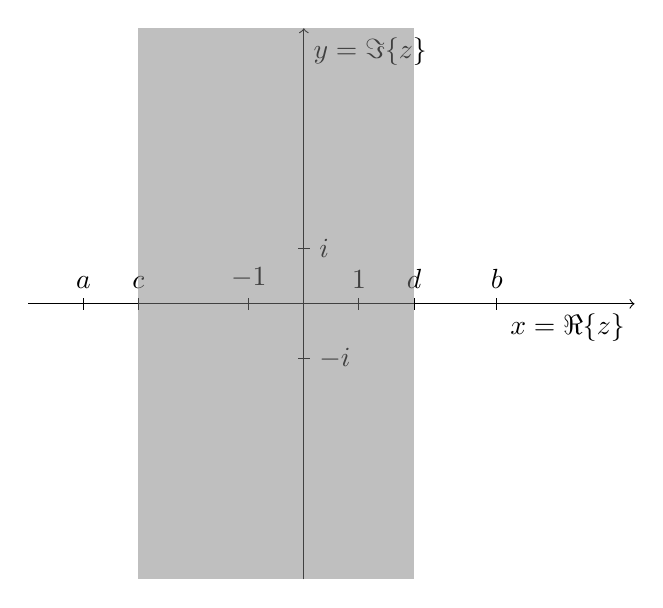
\begin{tikzpicture}
            \begin{scope}[scale=0.7]
            \draw [->] (-5,0) -- (6,0) node [below left]  {$x = \Re\{z\}$};
            \draw [->] (0,-5) -- (0,5) node [below right] {$y = \Im\{z\}$};
        
            \draw (1,-3pt) -- (1,3pt)   node [above] {$1$};
            \draw (-1,-3pt) -- (-1,3pt) node [above] {$-1$};
            \draw (-3pt,1) -- (3pt,1)   node [right] {$i$};
            \draw (-3pt,-1) -- (3pt,-1) node [right] {$-i$};
            \draw (-3,-3pt) -- (-3,3pt) node [above] {$c$};
            \draw (2,-3pt) -- (2,3pt) node [above] {$d$};
            \draw (-4,-3pt) -- (-4,3pt) node [above] {$a$};
            \draw (3.5,-3pt) -- (3.5,3pt) node [above] {$b$};

            \path [draw=none,fill=gray,semitransparent] (-3, -5) rectangle (2, 5);
            \end{scope}
        \end{tikzpicture}\]
        Since $f(z)$ is analytic in this domain, Cauchy's integral theorem tells us that:
        \[
            \oint_{C} f(z) \diff z = 0
        \]
        where $C$ is the boundary of $\Omega$. Splitting $C$ into four pieces:
        \begin{align*}
            \oint_C f(z) \diff z &= \lim_{y\to-\infty}\int_{c}^{d} f(x+iy) \diff x+ \int_{-\infty}^\infty f(d+iy) \diff y  \\
            &\mspace{35mu} + \lim_{y\to\infty} \int_{d}^c f(x+iy) \diff x + \int_{\infty}^{-\infty} f(c+iy) \diff y
        \end{align*}
        The horizontal pieces go to zero since $f\to 0$ on all vertical lines within the strip between $x=a$ and $x=b$. Splitting $f(x+yi) = F(x, y) + iG(x, y)$ into real and imaginary parts gives:
        \[
            \int_{-\infty}^{\infty} F(d, y) + iG(d, y) \diff y - \int_{-\infty}^{\infty} F(c, y) + iG(c, y) \diff y = 0
        \]
        Equating real parts gives:
        \[
            \int_{-\infty}^{\infty} F(d, y) \diff y = \int_{-\infty}^{\infty} F(c, y) \diff y
        \]
        Since $c$ and $d$ are chosen arbitrarily we must have that:
        \[
            \int_{-\infty}^{\infty} F(x,y) \diff y = \textnormal{const.} \qquad (a < x < b)
        \]
        \item Applying the result to $f(z) = e^{z^2}$ gives:
        \[
            \int_{-\infty}^{\infty} \Re\left( e^{(x+iy)^2} \right)\diff y = c \qquad (x,y \textnormal{ real})
        \]
        immediately giving the result:
        \[
            \int_{-\infty}^\infty e^{x^2}\cos(2xy)e^{-y^2} \diff y = c \Longleftrightarrow  \int_{-\infty}^\infty \cos(2xy)e^{-y^2} \diff y = ce^{-x^2}
        \]
        The constant can be found by plugging in $x=0$ and recognizing the classical Gaussian integral:
        \[
            \sqrt{\pi} = \int_{-\infty}^\infty e^{-y^2} \diff y = c
        \]
    \end{enumerate}
\end{solution}

\begin{exercise}
    This exercise gives a neat proof of Cayley's formula for the number of trees of $n$ vertices, by showing more, namely, that there is a pretty formula for the number of such trees even if the degrees of all vertices are specified.
    \begin{enumerate}[label=(\alph*)]
        \item Let $d_1, \ldots, d_n$ be positive integers whose sum is $2n-2$. Show that the number of vertex-labeled trees $T$ of $n$ vertices, in which for all $i=1,\ldots,n$ it is true that $d_i$ is the degree of vertex $i$ of $T$, is exactly 
        \[
            f_n(d_1,\ldots,d_n)=\frac{(n-2)!}{(d_1-1)!(d_2-1)!\cdots (d_n-1)!}
        \]
        (Do this by induction on $n$. show that one of the $d_i$'s, at least, must be $=1$ and go from there.)
        \item Find the generating function 
        \[
            F_n(x_1,\ldots,x_n) = \sum_{\substack{d_1+\cdots+d_n = 2n-2 \\ d_1,\ldots,d_n\geq 1}} f_n(d_1, \ldots, d_n)x_1^{d_1}\cdots x_n^{d_n}
        \]
        in a pleasant, explicit form, involving no summation signs.
        \item Let $x_1=x_2=\cdots=x_n=1$ in your answer to part (b), and thereby prove Cayley's result that there are exactly $n^{n-2}$ labeled trees of $n$ vertices.
        \item Use the sieve method to show that if $e_k$ is the number of vertex labeled trees on $n$ vertices of which $k$ are endpoints (vertices of degree $1$), then 
        \[
            \sum_k e_k x^k = \sum_r \binom{n}{r}r^{n-2}(x-1)^{n-r}
        \]
        \item Show that the average number of endpoints that trees of $n$ vertices have is
        \[
            n\left(1-\frac{1}{n}\right)^{n-2} \sim \frac{n}{e} \quad (n\to\infty)
        \]
        i.e., \emph{the probability that a random vertex of a tree is an endpoint is about $1/e$}.
    \end{enumerate}
\end{exercise}
\begin{solution}
    \begin{enumerate}[label=(\alph*)]
        \item \hypertarget{eq:ch4:18:a}{4.18(a)} Suppose that all $d_i$'s are greater than $1$, then their sum is:
        \[
            \sum_{i=1}^n d_i \geq \sum_{i=1}^n 2 = 2n
        \]
        which is a contradiction, since they have to sum to $2n-2$, hence at least one needs to have degree $1$ (actually, this proof even shows that there must be at least $2$ vertices with degree $1$).

        Now, we proceed by induction on $n$. The base case is obviously true, since there is only one labeled tree with $2$ vertices (with both vertices having degree $1$). 

        Let $n>2$ and assume the formula holds for $n-1$. Let $d_i$ be the vertex whose degree is $1$. This vertex must connect to one of the other vertices of degree $>1$. Let this connecting vertex have index $j$. Removing this edge and vertex $i$ leaves a tree on $n-1$ vertices with degrees $(d_1, \ldots, d_{i-1}, d_{i+1}, \ldots, d_j - 1, \ldots, d_n)$. Summing over all possible $j$ gives (using the formula for the number of labeled trees on $n-1$ vertices given a degree list by the induction hypothesis):
        \[
            f_n(d_1,\ldots,d_n) = \sum_{\substack{1\leq j\leq n \\ d_j \neq 1 \\ i \neq j}} \frac{(n-3)!}{(d_1-1)!\cdots (d_{i-1} - 1)! (d_{i+1} -1)!\cdots (d_j - 2)! \cdots}
        \]
        Multiplying numerator and denominator by $(d_j-1)$:
        \[
            f_n(d_1,\ldots,d_n) = \sum_{\substack{1\leq j\leq n \\ d_j \neq 1 \\ i \neq j}} \frac{(n-3)!(d_j-1)}{(d_1-1)!\cdots (d_{i-1} - 1)! (d_{i+1} -1)!\cdots (d_j - 1)! \cdots}
        \]
        Multiplying denominator by $(d_i-1)! = 1$:
        \[
            f_n(d_1,\ldots,d_n) = \sum_{\substack{1\leq j\leq n \\ d_j \neq 1 \\ i \neq j}} \frac{(n-3)!(d_j-1)}{(d_1-1)!\cdots (d_{i} - 1)!\cdots (d_j - 1)! \cdots (d_n-1)!}
        \]
        Relax the condition on $d_j\neq 1$ since including it in the sum gives a zero term anyway:
        \[
            f_n(d_1,\ldots,d_n) = \sum_{\substack{1\leq j\leq n \\ i \neq j}} \frac{(n-3)!(d_j-1)}{(d_1-1)!\cdots (d_{i} - 1)!\cdots (d_j - 1)! \cdots (d_n-1)!} 
        \]
        Factoring out the common part:
        \[
            f_n(d_1,\ldots,d_n) = \frac{(n-3)!}{(d_1-1)!(d_2-1)! \cdots (d_n-1)!} \sum_{\substack{1\leq j\leq n \\ i \neq j}}(d_j-1)
        \]
        The sum of the degrees is $2n-3$ since the vertex with degree $1$ (at index $i$) is excluded and we therefore get:
        \begin{align*}
            f_n(d_1,\ldots,d_n) &= \frac{(n-3)!}{(d_1-1)!(d_2-1)! \cdots (d_n-1)!} ((2n-3) - (n-1)) \\
            &=  \frac{(n-2)!}{(d_1-1)!(d_2-1)! \cdots (d_n-1)!}
        \end{align*}
        as desired.
        \item The generating function is:
        \[
            F_n(x_1,\ldots,x_n) = \sum_{\substack{d_1+\cdots+d_n = 2n-2 \\ d_1,\ldots,d_n\geq 1}} f_n(d_1, \ldots, d_n)x_1^{d_1}\cdots x_n^{d_n}
        \]
        Let $r_i = d_i - 1$ such that:
        \[
            F_n(x_1,\ldots,x_n) = \sum_{\substack{r_1+\cdots+r_n = n-2 \\ r_1,\ldots,r_n\geq0} } f_n(r_i+1, \ldots, r_n+1)x_1^{r_1+1}\cdots x_n^{r_n+1}
        \]
        Using the multinomial theorem:
        \begin{align*}
            F_n(x_1,\ldots,x_n) \estepalign{\hyperlink{4.18(a)}{4.18(a)}} (x_1x_2\cdots x_n)\sum_{\substack{r_1+\cdots+r_n = n-2 \\ r_1,\ldots,r_n\geq0} } \frac{(n-2)!}{r_1! r_2!\cdots r_n!} x_1^{r_1}\cdots x_n^{r_n} \\
            \estepalign{\ref{ex:2-20}} (x_1x_2\cdots x_n) (x_1+x_2+\ldots+x_n)^{n-2}
        \end{align*}
        \item Letting $x_1=x_2=\cdots=x_n = 1$ gives:
        \[
            \sum_{\substack{d_1+\cdots+d_n = 2n-2 \\ d_1,\ldots,d_n\geq 1}} f_n(d_1, \ldots, d_n) = (1\cdot1\cdots 1)(1+1+\ldots+1)^{n-2} = n^{n-2}
        \]
        \item Let $\Omega$ be the set of all labeled trees on $n$ vertices. There is a property $i$ if a tree has vertex $i$ as endpoint. Let $S$ be a set of endpoints. The number of trees which have all vertices in $S$ as endpoints is:
        \[
            N(\supseteq S) = (n-|S|)^{|S|}(n - |S|)^{n-|S|-2} = (n-|S|)^{n-2}
        \]
        The first factor comes from the possiblities for which each endpoint is connected to. The second term is the number of labeled trees on $(n-|S|)$ vertices. To visualize this construction, start with an arbitrary tree of $(n-|S|)$ vertices, then choose $|S|$ of these vertices (with each vertex possibly chosen multiple times) and then connect the set of endpoints in $S$ to these vertices.
        
        The unfiltered data is therefore:
        \[
            N_r = \sum_{|S| = r} N(\supseteq S) = \binom{n}{r} (n-r)^{n-2}
        \]
        By the sieve method:
        \[
            \bsum[k]  e_k x^k = E(x) \estep{\eqref{eq:sieve}} N(x-1) = \bsum[r] \binom{n}{r} (n-r)^{n-2}(x-1)^r
        \]
        After a change of variables
        \[
            \bsum[k]  e_k x^k = \bsum[r] \binom{n}{r} r^{n-2}(x-1)^{n-r}
        \]
        \item The average number of endpoints is given by $E'(1) / E(1)$ which is equal to:
        \begin{align*}
            \frac{E'(1)}{E(1)} = \frac{\binom{n}{n-1}(n-1)^{n-2}}{\binom{n}{n}n^{n-2}} = n\left(1 - \frac{1}{n}\right)^{n-2}  \sim n e^{-1} = \frac{n}{e}
        \end{align*}
    \end{enumerate}
\end{solution}

\begin{exercise}
    \begin{enumerate}[label=(\alph*)]
        \item If $N(\subseteq S)$ is the number of objects whose set of properties is contained in $S$, then for all sets $T$, the number of objects whose set of properties is \emph{precisely} $T$ is
        \[
            N(=T) = \sum_{S\subseteq T} (-1)^{|S| - |T|} N(\subseteq S)
        \]
        \item Let $S$ be a fixed set of positive integers, and let $h_n(S)$ be the number of hands of weight $n$, in a certain labeled exponential family, whose card sizes all belong to $S$. Find the egf of $\{h_n(S)\}$.
        \item Multiply by $(-1)^{|S|-|T|}$ and sum over $S\subseteq T$ to find the egf of $\{\psi_n(T)\}_{n\geq0}$, the number of hands whose set of distinct card sizes is \emph{exactly} $T$, in the form (the $d$'s are the deck sizes)
        \[
            \sum_{n\geq0} \frac{\psi_n(T)}{n!} x^n = \prod_{t\in T} \left(e^{\frac{d_tx^t}{t!}} - 1 \right)
        \]
        \item Let $\rho(n,k)$ be the number of hands of weight $n$ that have exactly $k$ different \emph{sizes} of cards (however many cards they might have!). Sum the result of (c) over all $|T|=k$, etc., to find that 
        \[
            \sum_{n,k\geq0} \frac{\rho(n,k)}{n!} x^n y^k = \prod_{t\geq1}\left\{1+y\left(e^{d_tx^t/t!}-1\right)\right\}
        \]
        \item Let $c_n$ be the average number of different sizes of cycles that occur in permutations of $n$ letters. Show that the opsgf of $\{c_n\}$ is 
        \[
            \frac{1}{1-x}\sum_{t\geq1} \left(1-e^{-x^t/t}\right)
        \]
        and find an explicit formula for $c_n$.
    \end{enumerate}
\end{exercise}
\begin{solution}
    \begin{enumerate}[label=(\alph*)]
        \item \hypertarget{eq:ch4:19:a}{} Note that:
        \[
            N(\subseteq S) = \sum_{U \subseteq S} N(=U)
        \]
        Starting from the right-hand side, we then have:
        \begin{align*}
            \sum_{S\subseteq T} (-1)^{|S| - |T|} N(\subseteq S) &= \sum_{S\subseteq T} (-1)^{|S| - |T|}\sum_{U \subseteq S} N(=U) \\
            &= \sum_{U \subseteq T} N(=U)  \sum_{U\subseteq S\subseteq T}(-1)^{|S| - |T|}
        \end{align*}
        Note that the inner sum can be rewritten as looping over all subsets $W$ of $T\setminus U$ (and compensating $|S|$ to be $|W| + |U|$):
        \[
            \sum_{S\subseteq T} (-1)^{|S| - |T|} N(\subseteq S) =  \sum_{U \subseteq T} N(=U) (-1)^{|U| - |T|} \sum_{W \subseteq T \setminus U}(-1)^{|W|}
        \]
        The inner sum is equivalent to:
        \[
            \sum_{W \subseteq T \setminus U}(-1)^{|W|} = \sum_{r=0}^{|T|-|U|} \binom{|T| - |U|}{r} (-1)^r
        \]
        which is $0$ for $|T| - |U| \neq 0$ by the binomial theorem and $1$ if $|T| - |U| = 0$:
        \[
            \sum_{W \subseteq T \setminus U}(-1)^{|W|} = \delta_{|T|, |U|}
        \]
        Plugging this back in yields:
        \[
            \sum_{S\subseteq T} (-1)^{|S| - |T|} N(\subseteq S) =  \sum_{U \subseteq T} N(=U) (-1)^{|U| - |T|} \delta_{|T|, |U|}
        \]
        But the only subset of $|T|$ which has the same size as $|T|$ is $|T|$ itself:
        \[
            \sum_{S\subseteq T} (-1)^{|S| - |T|} N(\subseteq S) = N(=T)(-1)^{|T|-|T|} = N(=T)
        \]
        \item \hypertarget{eq:ch4:19:b}{} Consider the same exponential family with only the $d_s$ where $s\in S$. Its deck enumerator is:
        \[
            \mathcal{D}_S(x) = \sum_{s\in S} d_s \frac{x^s}{s!}
        \]
        From the exponential formula, we then have:
        \begin{align*}
            \bsum[n] h_n(S) \frac{x^n}{n!} = \exp(\mathcal{D}_S(x)) = \prod_{s\in S} \exp\left(d_s \frac{x^s}{s!} \right)
        \end{align*}
        \item \hypertarget{eq:ch4:19:c}{} Multiplying by $(-1)^{|S|-|T|}$ and summing over $S\subseteq T$ gives:
        \[
            \sum_{S\subseteq T}\bsum (-1)^{|S|-|T|}h_n(S) \frac{x^n}{n!} \estep{\hyperlink{eq:ch4:19:b}{4.19(b)}} \sum_{S\subseteq T} (-1)^{|S|-|T|} \prod_{s\in S} \exp\left(d_s \frac{x^s}{s!} \right)
        \]
        The left-hand side of this equality is just the egf of $\{\psi_n(T)\}_{n\geq0}$ by part \hyperlink{eq:ch4:19:a}{4.19(a)}. Now we show that the right-hand side is:
        \[
            \prod_{t\in T} \left(\exp\left(\frac{d_tx^t}{t!}\right) - 1\right)
        \]
        by induction on the size of $|T|$.

        For the base case, let $T = \{t_1\}$ be a set of one element. Then we have that:
        \begin{align*}
            \sum_{S\subseteq T} (-1)^{|S|-|T|} \prod_{s\in S} \exp\left(\frac{d_s x^s}{s!} \right) &= (-1)^{0}\prod_{s\in \{t_1\}} \exp\left( \frac{d_tx^t}{t!}\right) + (-1)^{-1} \cdot 1 \\
            &= \prod_{t\in T}\left(\exp\left(\frac{d_tx^t}{t!}\right) - 1\right)
        \end{align*}
        where we used the fact that there are only two subsets of $T$ in the first equality. For ease of notation, let:
        \[
            P(S) = \prod_{s\in S} \exp\left(\frac{d_s x^s}{s!}\right)
        \]
        Now let $T$ be a set of $n$ elements and assume that 
        \[
            \sum_{S\subseteq T'} (-1)^{|S|-|T'|} P(S) = \prod_{t\in T'} \left(\exp\left(\frac{d_tx^t}{t!}\right) - 1\right)
        \]
        for any set $T'$ of $n-1$ elements.
        We do this by splitting the sum in subsets which contain $t_1$ and subsets which do not contain $t_1$ (where $t_1\in T$):
        \begin{align*}
            \sum_{S\subseteq T} (-1)^{|S|-|T|} P(S) &= \sum_{S\subseteq T\setminus \{t_1\}} (-1)^{|S| + 1 - |T|} \exp\left(\frac{d_{t_1}x^{t_1}}{t_1!}\right)P(S)\\
            &\mspace{50mu}+  \sum_{S\subseteq T\setminus \{t_1\}} (-1)^{|S| - |T|} P(S) \\
            &= \exp\left(\frac{d_{t_1}x^{t_1}}{t_1!}\right) \sum_{S\subseteq T'} (-1)^{|S| - |T'|} P(S)  \\
            &\mspace{50mu} - \sum_{S\subseteq T'} (-1)^{|S| - |T'|} P(S)
        \end{align*}
        Where $T' = T\setminus \{t_1\}$. Applying the induction hypothesis gives the desired result:
        \begin{align*}
            \sum_{S\subseteq T} (-1)^{|S|-|T|} P(S) &= \left(\exp\left(\frac{d_{t_1}x^{t_1}}{t_1!}\right) - 1\right)\prod_{t\in T'} \left(\exp\left(\frac{d_tx^t}{t!}\right) - 1\right) \\
            &=\prod_{t\in T} \left(\exp\left(\frac{d_tx^t}{t!}\right) - 1\right)
        \end{align*}
        We have therefore shown that:
        \[
            \bsum \frac{\psi_n(T)}{n!} x^n = \prod_{t\in T} \left(\exp\left(\frac{d_tx^t}{t!}\right) - 1 \right)
        \]
        \item Summing the result of part (c) over all $|T| = k$, multiplying by $y^k$ and summing over $k$:
        \[
            \bsum[k] \sum_{|T| = k} \bsum[n] \frac{\psi_n(T)}{n!}x^ny^k =\bsum[k] \sum_{|T|=k} \left\{\prod_{t\in T}\left(e^{\frac{d_tx^t}{t!}} - 1 \right)\right\}y^k
        \]
        On the left side we can use $\sum_{|T| = k} \psi_n(T) = \rho(n,k)$. For the right-hand side we start by moving $y$ inside (using $|T|=k$):
        \[
            \bsum[k] \sum_{|T|=k} \left\{\prod_{t\in T}\left(e^{\frac{d_tx^t}{t!}} - 1 \right)\right\}y^k = \bsum[k] \sum_{|T|=k} \left\{\prod_{t\in T}y\left(e^{\frac{d_tx^t}{t!}} - 1 \right)\right\}
        \]
        but the two summations just sum over all possible sets which can also be written as:
        \[
            \bsum[k] \sum_{|T|=k} \left\{\prod_{t\in T}y\left(e^{\frac{d_tx^t}{t!}} - 1 \right)\right\} = \prod_{t=1}^\infty \left\{ 1+y\left(e^{d_tx^t/t!} - 1\right)\right\}
        \]
        which has the semantics of either not choosing an element (the $1$) or choosing an element (the term with $y$). The result now follows:
        \[
            \bsum[n]\bsum[k] \rho(n,k) \frac{x^n}{n!} y^k = \prod_{t=1}^\infty\left\{1+y\left(e^{d_tx^t/t!}-1\right)\right\}
        \]
        \item In the exponential family for permutations and their cycles, we have $d_n = (n-1)!$ and therefore by the previous part:
        \[
            \bsum[n]\bsum[k] \frac{\rho(n,k)}{n!} x^n y^k = \prod_{t=1}^\infty\left\{1+y\left(\exp\left(\frac{x^t}{t}\right)-1\right)\right\}
        \]
        which is the enumerator for the number of permutations of $n$ letters with $k$ different cycles. Now taking the derivative with respect to $y$ and evaluating at $y=1$ gives exactly the opsgf of $c_n$ on the left-hand side:
        \[
            \bsum[n]\bsum[k] k\frac{\rho(n,k)}{n!} x^n = \bsum[n] c_n x^n = C(x)
        \]
        Applying the same operation to the right-hand side:
        \begin{align*}
            C(x) &= \frac{\partial}{\partial y} \prod_{t=1}^\infty\left\{1+y\left(\exp\left(\frac{x^t}{t}\right)-1\right)\right\}\bigg\rvert_{y=1} \\
            &= \sum_{t=1}^\infty \left(\exp\left(\frac{x^t}{t}\right)-1\right) \prod_{\substack{t'\geq 1\\ t'\neq t}}\left\{1+y\left(\exp\left(\frac{x^{t'}}{t'}\right)-1\right)\right\}\bigg\rvert_{y=1} 
            \\
            &= \sum_{t=1}^\infty \left(\exp\left(\frac{x^t}{t}\right)-1\right) \prod_{\substack{t'\geq 1\\ t'\neq t}}\left\{\exp\left(\frac{x^{t'}}{t'}\right)\right\}
        \end{align*}
        where we used the product rule for differentiation in the second equality. Working this out further yields
        \begin{align*}
            C(x) &=  \sum_{t=1}^\infty \left(\exp\left(\frac{x^t}{t}\right)-1\right) \exp\left(-\frac{x^t}{t}\right)\prod_{t'= 1}^\infty\left\{\exp\left(\frac{x^{t'}}{t'}\right)\right\} \\
            &= \sum_{t=1}^\infty \left(\exp\left(\frac{x^t}{t}\right)-1\right) \exp\left(-\frac{x^t}{t}\right)\exp\left\{{\sum_{t'=1}^\infty \frac{x^{t'}}{t'}}\right\}
        \end{align*}
        In the exponent, the power series of $\log \frac{1}{1-x}$ is recognized, see \eqref{eq:power_loggeom}, yielding:
        \[
            C(x) = \frac{1}{1-x}\sum_{t=1}^\infty \left(1-\exp\left(-\frac{x^t}{t}\right)\right)
        \]
        For an explicit formula for $c_n$ we need to extract the coefficient of $x^n$. Since multiplying by $\frac{1}{1-x}$ extracts the sequence of partial sums, we are interested in:
        \[
            c_n = \sum_{j=0}^n \coeff{x^j} \sum_{t= 1}^\infty \left(1-\exp\left(-\frac{x^t}{t}\right)\right)
        \]
        The coefficient of $x^j$ is given by:
        \begin{align*}
            \coeff{x^j} \sum_{t=1}^\infty \left(1-\exp\left(-\frac{x^t}{t}\right)\right) \estepalign{\eqref{eq:power_exp}} \coeff{x^j} \sum_{t=1}^\infty \sum_{k= 1}^\infty \frac{(-1)^{k+1}x^{kt}}{t^k k!} \\
            &= \begin{cases}
                \sum_{m|j} \frac{(-1)^{m+1}}{(j/m)^m m!} & j\neq 0 \\
                0 & j = 0
            \end{cases}
        \end{align*}
        such that:
        \[
            c_n = \sum_{j=1}^n \sum_{m\vert j} \frac{(-1)^{m+1}}{(j/m)^m m!}
        \]
    \end{enumerate}
\end{solution}

\begin{exercise}
    Begin with the set $\{1, 2, \ldots, n\}$. Toss a coin $n$ times, once for each member of the set. Keep the elements that scored `Heads' and discard the elements that got `Tails'. You now have a certain subset $S$ of the original set. Call this whole process a `step'. Now take a step from $S$. That is, toss a coin for each element of $S$, and keep those that get `Heads', getting a sub-subset $S'$, etc.\ The game halts when the empty set is reached. Let $f(n,k,r)$ be the probability that after $k$ steps, exactly $r$ objects remain.
    \begin{enumerate}[label=(\alph*)]
        \item Find a recurrence relation for $f$, find the generating function for $f$, and find $f$ itself.
        \item What is the \emph{average} number of steps in a complete game?
        \item What is the standard deviation of the number of steps in the game?
    \end{enumerate}
\end{exercise}
\begin{solution}
    \begin{enumerate}[label=(\alph*)]
        \item The probability that after $k$ steps exactly $r$ coins remain starting with $n$ coins is the following sum (advance from $k-1$ to $k$, choose a subset of size $r$, toss heads for all of these, toss heads for the rest, multiply by the possible number of ways):
        \[
            f(n,k,r) = \sum_{r'=r}^{n} f(n, k - 1, r') \binom{r'}{r} \frac{1}{2^{r'}} =  \bsum[r'] f(n, k - 1, r') \binom{r'}{r} \frac{1}{2^{r'}}
        \]
        for $k\geq 1$, where we used the fact that $\binom{n}{k} = 0$ for $n < k$ as well as $f(n,k-1,r') = 0$ for $r'>n$. At $k=0$, we have the following identity:
        \[
            f(n,0,r) = \delta_{n,r}
        \]
        Define $F_{k,r}(x) = \bsum f(n,k,r) x^n$ and note that $F_{0,r}(x) = x^r$. Multiplying both sides of the recurrence by $x^n$ and summing over $n$ gives:
        \[
            F_{k,r}(x) = \bsum[n] \bsum[r'] f(n,k-1,r') \binom{r'}{r} \frac{1}{2^{r'}} x^n = \bsum[r'] F_{k-1,r'} \binom{r'}{r} \frac{1}{2^{r'}}
        \]
        Starting from:
        \[ 
            F_{0,r} = x^r 
        \]
        we then get:
        \[
            F_{1,r} = \bsum[r'] \left(\frac{x}{2}\right)^{r'} \binom{r'}{r} \estep{\eqref{eq:binom_denom_num_single}} \frac{\left(\frac{x}{2}\right)^r}{\left(1-\frac{x}{2}\right)^{r+1}} = \frac{2}{2-x} \left(\frac{x}{2-x}\right)^{r}
        \]
        \begin{align*}
            F_{2,r} &= \frac{2}{2-x}\bsum[r'] \left(\frac{x}{2-x}\right)^{r'} \binom{r'}{r} \frac{1}{2^{r'}} \estep{\eqref{eq:binom_denom_num_single}} \frac{2}{2-x} \frac{\left(\frac{x}{4-2x}\right)^r}{\left(1-\frac{x}{4-2x}\right)^{r+1}} \\
            &= \frac{2}{2-x}\frac{4-2x}{4-3x} \left(\frac{x}{4-3x}\right)^{r} = \frac{4}{4-3x}\left(\frac{x}{4-3x}\right)^{r}
        \end{align*}
        This suggests a general form:
        \[
            F_{k,r}(x) = \frac{2^{k}}{2^k - (2^k - 1)x}\left(\frac{x}{2^k - (2^k-1)x}\right)^r = \frac{2^k x^r}{(2^k - (2^k-1)x)^{r+1}}
        \]
        We show this by induction on $k$:
        \begin{align*}
            F_{k,r} &= \frac{2^{k-1}}{2^{k-1} - (2^{k-1} - 1)x} \bsum[r'] \left(\frac{x}{2^{k-1} - (2^{k-1}-1)x}\right)^{r'} \binom{r'}{r} \frac{1}{2^{r'}} \\
            &=\frac{2^{k-1}}{2^{k-1} - (2^{k-1} - 1)x} \bsum[r'] \left(\frac{x}{2^{k} - (2^{k}-2)x}\right)^{r'} \binom{r'}{r} \\
            \estepalign{\eqref{eq:binom_denom_num_single}} \frac{2^{k-1}}{2^{k-1} - (2^{k-1} - 1)x} \left(\frac{\left(\frac{x}{2^k-(2^k - 2)x}\right)^r}{\left(1-\frac{x}{2^k-(2^k-2)x}\right)^{r+1}}\right) \\ 
            &= \frac{2^{k-1}}{2^{k-1} - (2^{k-1} - 1)x} \frac{2(2^{k-1} - (2^{k-1}-1)x)}{2^k - (2^k -1)x}\left(\frac{x}{2^k - (2^k-2)x - x}\right)^r \\
            &= \frac{2^k}{2^k - (2^k - 1)x} \left(\frac{x}{2^k - (2^k-1)x}\right)^r \\
            &=  \frac{2^k x^r}{(2^k - (2^k-1)x)^{r+1}}
        \end{align*}
        $f(n,k,r)$ is then easily found from taking the coefficient $\coeff{x^n}F_{k,r}(x)$:
        \begin{align*}
            f(n,k,r) &= \coeff{x^{n-r}} \frac{2^{k}}{2^{k(r+1)} (1 - (1-2^{-k})x)^{r+1}} \\
            \estepalign{\eqref{eq:binom_denom}} 2^{-kr} \coeff{x^{n-r}} \infsum[m] \binom{m+r}{m} (1-2^{-k})^m x^m \\
            &= 2^{-kr} \binom{n}{n-r}(1-2^{-k})^{n-r}
        \end{align*}
        \item To calculate the average, we first calculate the probability that a game ends after $k$ tosses. This is given by:
        \[
            p_{n}(k) = \sum_{r=1}^\infty f(n, k-1, r) \frac{1}{2^r}
        \]
        since in the last step all coins must be eliminated.
        
        Working this out with the previously found formula gives:
        \begin{align*}
            p_n(k) &= \sum_{r=1}^n 2^{-(k-1)r} \binom{n}{n-r} (1-2^{-k+1})^{n-r} 2^{-r} \\
            &= \sum_{r=1}^n \binom{n}{n-r} \left(2^{-k}\right)^r (1-2^{-k+1})^{n-r}
        \end{align*}
        This is just the binomial theorem \eqref{eq:binom_num2} where the term with $r=0$ is omitted:
        \begin{align*}
            p_n(k) &= \left(1-2^{-k+1} + 2^{-k}\right)^n - \left(1-2^{-k+1}\right)^n \\
            &= \left(1-2^{-k}\right)^n - \left(1-2^{-k+1}\right)^n
        \end{align*}
        The average number of steps to complete the game is now given by:
        \[
            \mu_n = \bsum[k] kp_n(k) = \bsum[k] k \left\{\left(1-2^{-k}\right)^n - \left(1-2^{-k+1}\right)^n \right\}
        \]
        To get a finite summation, we use a different formulation. Let $X$ be the random variable denoting the number of steps in a game. Since $X$ is positive, we can use:
        \[
            \mu_n = \bsum[k] P(X > k)
        \]
        The probability that $X > k$ is given by:
        \[
           P(X > k) = 1 - f(n, k, 0)
        \]
        since $f(n, k, 0)$ gives the probability that the game has ended after the $k$th turn. Filling this in, we get:
        \begin{align*}
            \mu_n &= \bsum[k] 1 - f(n,k,0) = \bsum[k] 1 - (1-2^{-k})^n \estep{\eqref{eq:binom_num}} \bsum[k] \sum_{m=1}^n \binom{n}{m} \frac{(-1)^{m+1}}{2^{mk}} \\
            &= \sum_{m=1}^n \binom{n}{m} (-1)^{m+1}  \bsum[k] 2^{-mk} \estep{\eqref{eq:power_geom}} \sum_{m=1}^n \binom{n}{m} (-1)^{m+1} \frac{1}{1-2^{-m}}
        \end{align*}
        Both of these formulations can also be found in \href{https://oeis.org/A158466}{OEIS A158466}.
        \item The variance is given by:
        \[
            \sigma^2_n = \left\{\bsum[k] k^2 p_n(k)\right\} - \mu^2_n
        \]
        where the first term is
        \[
            \bsum[k] k^2 p_n(k) = \bsum[k] k^2 \left\{(1-2^{-k})^n - (1-2^{-k+1})^n\right\}
        \]
        Again, we can formulate a finite sum by using the identity
        \[
            \bsum[k] k^2 p_n(k) = \bsum[k] (2k+1)P(X > k)
        \]
        where $\bsum[k] P(X>k)$ has already been calculated in the previous part and we only require
        \[
            \bsum[k] 2k P(X > k) = \bsum[k] 2k(1-f(n,k,0)) = \bsum[k] 2k (1 - (1-2^{-k})^n)
        \]
        which we find from a similar calculation:
        \begin{align*}
            \bsum[k] 2k P(X>k) \estepalign{\eqref{eq:binom_num}} \bsum[k] 2k \sum_{m=1}^n \binom{n}{m} \frac{(-1)^{m+1}}{2^{mk}} \\
            &= \sum_{m=1}^n 2 \binom{n}{m} (-1)^{m+1} \bsum[k] \frac{k}{2^{mk}} x^k \bigg\rvert_{x=1} \\
            \estepalign{\eqref{eq:xD}} \sum_{m=1}^n 2 \binom{n}{m}(-1)^{m+1} xD \bsum[k] \left(\frac{x}{2^m}\right)^k \bigg\rvert_{x=1} \\
            \estepalign{\eqref{eq:power_geom}} \sum_{m=1}^n2\binom{n}{m}(-1)^{m+1} xD\frac{1}{1 - x2^{-m}}\bigg\rvert_{x=1} \\
            &= \sum_{m=1}^n \binom{n}{m}(-1)^{m+1} \frac{2\cdot 2^{m}}{(2^m-1)^2}
        \end{align*}
        To conclude, we have that:
        \begin{align*}
            \bsum[k] k^2 p_n(k) &= \sum_{m=1}^n \binom{n}{m} (-1)^{m+1} \left\{\frac{2^{m+1}}{(2^m - 1)^2} + \frac{1}{1-2^{-m}} \right\} \\
            &= \sum_{m=1}^n \binom{n}{m} (-1)^{m+1} \frac{2^m - 4^m}{(2^m - 1)^2}
        \end{align*}
        and the standard deviation given by
        \[
            \sigma_n = \sqrt{\sum_{m=1}^n \left[\binom{n}{m} (-1)^{m+1} \frac{2^m - 4^m}{(2^m - 1)^2}\right] -\left[\sum_{m=1}^n \binom{n}{m} (-1)^{m+1} \frac{2^m}{2^m-1}\right]^2}
        \]
    \end{enumerate}
\end{solution}

\begin{exercise}
    Let $f(n,k,t)$ be the number of HC-polyominoes that have $n$ cells, in $k$ layers, the highest layer consisting of exactly $t$ cells. Show that the `grand' three-variable generating function is
    \[
        \sum_{n,k,t} f(n,k,t)x^ny^kz^t = \frac{xyz(1-x)^2((1-xz)(1-x)^2+x^2y(z-1))}{(1-xz)^2((1-x)^4-xy(1-x-x^2+x^3+x^2y))}
    \]
\end{exercise}
\begin{solution}
    We first list the known results which we will use (see the main text for the derivations). Denote $F_{k,t}(x) = \sum_n f(n,k,t)x^n$ with $F_{1,t} = x^t$ which satisfies:
    \[
        F_{k,t}(x) = x^t (V_{k-1}(x) +(t-1)U_{k-1}(x)) \qquad (k\geq 2)
    \]
    where $U_k(x) = \sum_{r=1}^\infty F_{k,r}(x)$ and $V_k(x)= \sum_{r=1}^\infty rF_{k,r}(x)$ with initial values $U_1(x) = x/(1-x)$, $V_1(x) = x/(1-x)^2$ and $U_0(x) = V_0(x) = 0$. These satisfy the simultaneous recurrences:
    \begin{align*}
        U_k(x) &= \frac{x}{1-x} V_{k-1}(x) + \frac{x^2}{(1-x)^2}U_{k-1}(x)  \qquad\mspace{3mu}(k\geq 2) \\
        V_k(x) &= \frac{x}{(1-x)^2}V_{k-1}(x) + \frac{2x^2}{(1-x)^3}U_{k-1}(x)\quad  (k\geq 2)
    \end{align*}
    We also have the generating function:
    \[
        \phi(x,y) = \bsum[k] U_k(x)y^k = \frac{xy(1-x)^3}{(1-x)^4-xy(1-x-x^2+x^3+x^2y)}
    \]
    Now define the generating function:
    \[
        \psi(x, y) = \bsum[k] V_k(x)y^k
    \]
    which we find by multiplying the recurrence for $U_k(x)$ by $y^k$ and summing over $k\geq 2$:
    \[
        \phi(x,y) - \frac{xy}{1-x} = \frac{xy}{1-x}\psi(x,y) + \frac{x^2y}{(1-x)^2}\phi(x,y)
    \]
    Solving for $\psi(x,y)$ gives:
    \[
        \psi(x,y) = \left(\frac{(1-x)^2 -x^2y}{xy(1-x)}\right)\phi(x,y) - 1
    \]
    Multiplying the recurrence for $F_{k,t}(x)$ by $y^kz^t$ and summing over $k\geq 2$ and $t\geq 1$ yields:
    \[
        \sum_{k=2}^\infty\sum_{t=1}^\infty F_{k,t}(x)y^kz^t =\sum_{k=2}^\infty\sum_{t=1}^\infty x^t(V_{k-1}(x) + (t-1)U_{k-1}(x))y^kz^t
    \]
    We rewrite the left-hand side in terms of the wanted generating function:
    \begin{align*}
        \textnormal{l.h.s.} &= \sum_{t=1}^\infty\sum_{k=1}^\infty F_{k,t}(x)y^kz^t  - \sum_{t=1}^\infty F_{1,t}(x)yz^t \\
        &= \sum_{t=1}^\infty\sum_{k=1}^\infty F_{k,t}(x)y^kz^t - \sum_{t=1}^\infty x^tyz^t \\
        \estepalign{\eqref{eq:power_geom}} F(x,y,z) - \frac{y}{1-xz} + y  \\
        &= F(x,y,z) - \frac{xyz}{1-xz}
    \end{align*}
    where we also used the fact that $f(n,k,t)=0$ whenever $k=0$ or $t=0$.
    For the right side, swap the summations to recognize $\psi(x,y)$ and $\phi(x,y)$:
    \begin{align*}
        \textnormal{r.h.s.} &= \sum_{t=1}^\infty x^tz^t \bigg\{\sum_{k=2}^\infty V_{k-1}(x)y^k + (t-1)\sum_{k=2}^\infty U_{k-1}(x)y^k\bigg\} \\
        &=\sum_{t=1}^\infty x^tz^t \left(y\psi(x,y) + (t-1)y\phi(x,y)\right) \\
        &= \frac{xyz}{1-xz}\psi(x,y) + \frac{xyz}{(1-xz)^2}\phi(x,y) - \frac{xyz}{1-xz}\phi(x,y)\\
        &=  \frac{xyz}{1-xz}\psi(x,y) + \frac{yx^2z^2}{(1-xz)^2} \phi(x,y) 
    \end{align*}
    where in the third equality we used the identities
    \[
        C\sum_{t=1}^\infty x^tz^t \estep{\eqref{eq:power_geom}} C \left(\frac{1}{1-xz} - 1\right) = \frac{Cxz}{1-xz}
    \]
    and
    \[
        C\sum_{t=1}^\infty tx^tz^t \estep{\eqref{eq:xD}} C xD_x\sum_{t=1}^\infty x^tz^t = xD_x \frac{Cxz}{1-xz} = \frac{Cxz}{(1-xz)^2}
    \]
    where $C$ is an expression which is constant with respect to $t$ and $D_x$ denotes differentation with respect to $x$.
    Combining this with the left-hand side, we obtain:
    \[
        F(x,y,z) = \frac{xyz}{1-xz}(\psi(x,y) + 1) + \frac{yx^2z^2}{(1-xz)^2} \phi(x,y)
    \]
    We start by filling in $\psi(x,y)$ and doing some algebraic manipulations:
    \begin{align*}
        F(x,y,z) &= \frac{xyz}{1-xz} \left\{\left(\frac{(1-x)^2 -x^2y}{xy(1-x)}\right)\phi(x,y) - 1 + 1\right\}  + \frac{yx^2z^2}{(1-xz)^2} \phi(x,y) \\
        &= \frac{z(1-x)^2 -x^2yz}{(1-xz)(1-x)}\phi(x,y) + \frac{yx^2z^2}{(1-xz)^2}\phi(x,y) \\
        &= \frac{(1-xz) \left(z(1-x)^2 - x^2yz\right)+ yx^2z^2 - yx^3z^2}{(1-xz)^2(1-x)}\phi(x,y) \\
        &= \frac{z((1-xz)(1-x)^2 - (1-xz)x^2y + yx^2z -yx^3z)}{(1-xz)^2(1-x)}\phi(x,y) \\
        &= \frac{z((1-xz)(1-x)^2 + x^2y(z-1))}{(1-xz)^2(1-x)}\phi(x,y)
    \end{align*}
    Lastly, we fill in $\phi(x,y)$ to obtain the final result:
    \begin{align*}
        F(x,y,z) &= \frac{z((1-xz)(1-x)^2 + x^2y(z-1))\left\{xy(1-x)^3\right\}}{(1-xz)^2(1-x) \left\{(1-x)^4-xy(1-x-x^2+x^3+x^2y) \right\}} \\
        &= \frac{xyz(1-x)^2((1-xz)(1-x)^2+x^2y(z-1))}{(1-xz)^2((1-x)^4-xy(1-x-x^2+x^3+x^2y))}
    \end{align*}
\end{solution}

\begin{exercise}
    Let $(a_1, b_1)$, \ldots, $(a_k, b_k)$ be an exact covering sequence. Show that 
    \[
        \sum_{j : a_j \textnormal{ is even}} \frac{1}{b_j} = \frac{1}{2} = \sum_{j : a_j \textnormal{ is odd}} \frac{1}{b_j}
    \]
    Generalize this result to other residue classes for the $a_j$.
\end{exercise}
\begin{solution}
    The statement is incorrect, consider the ECS $\{(0, 3)$, $(1, 3)$, $(2, 3)\}$.

    However if all $b_j$ are even, the statement does hold. Indeed, since the polynomial $\psi_2(z) = \sum_{j:2\vert b_j} \frac{z^{a_j}}{b_j} = \sum_{j=1}^k \frac{z^{a_j}}{b_j}$ is divisible by the cyclotomic polynomial $\Phi_2(z)$, we find that:
    \[
        \psi_2(-1) = \sum_{j=1}^k \frac{(-1)^{a_j}}{b_j} = \sum_{j:a_j \textnormal{ is even}} \frac{1}{b_j} -  \sum_{j:a_j \textnormal{ is odd}} \frac{1}{b_j} = 0
    \]
    and since $\sum_{j=1}^k \frac{1}{b_j} = 1$, the result follows.

    For general residue classes of $a_j$, let every $b_j$ be divisble by $n$. Then the polynomial
    \[
        \psi_n(z) = \sum_{j:n \vert b_j} \frac{z^{a_j}}{b_j} = \sum_{j=1}^k \frac{z^{a_j}}{b_j}
    \]
    is divisble by $\Phi_n(z)$. Evaluating this at the roots of unity, together with the fact that$ \sum_{j=1}^k \frac{1}{b_j} = 1$ gives rise to the equations:
    \[
        \begin{pmatrix}
            1 & 1 & \cdots & 1 \\
            1 & \omega_n^1 & \cdots & \omega_n^{n-1} \\
            \vdots & \vdots &\ddots & \vdots \\
            1 & \omega_n^{n-1} & \cdots & \omega_n^{(n-1)(n-1)}
        \end{pmatrix} \begin{pmatrix}
            x_0 \\ x_1 \\ \vdots \\ x_{n-1}
        \end{pmatrix} = \begin{pmatrix}
            1 \\ 0 \\ \vdots \\ 0
        \end{pmatrix}
    \]
    where
    \[
        x_i = \sum_{j: a_j \bmod n = i} \frac{1}{b_j}
    \]
    This matrix is just the DFT and inverting gives the desired result:
    \[
        x_0 = x_1 = \cdots = x_{n-1} = \frac{1}{n}
    \]
    (first column of IDFT matrix).
\end{solution}

\begin{exercise}
    What is the probability that a random permutation has equal number of $r$-cycles and $s$-cycles? Express your answer in terms of Bessel functions. Make a table of your answer, as a function of $r$ and $s$, for $1 < r < s \leq 6$.
\end{exercise}
\begin{solution}
    The probability that a random permutation has exactly $j$ $r$-cycles and $j$ $s$-cycles is:
    \[
        \frac{e^{-1/r-1/s}}{r^{j}s^j j!^2}
    \]
    The required probability is then found by summing over all $j$.
    \[
        e^{-1/r-1/s} \sum_{j=0}^\infty \frac{1}{(rs)^j j!^2} = e^{-1/r-1/s} I_0\left(\frac{2}{\sqrt{rs}}\right)
    \]
    where $I_0$ is the modified Bessel function of the first kind:
    \[
        I_0(z) = \sum_{k=0}^\infty \frac{\left(\frac{1}{4}z^2\right)^k}{(k!)^2}
    \]
    Some values are listed in following Table:
    \begin{table}[hbpt]
        \centering
        \begin{NiceTabular}{@{}wr{0.3cm}rrrrr@{}}
            \toprule
            \diagbox{$r$}{$s$} & $2$ & $3$ & $4$ & $5$ & $6$ \\ \midrule
            $1$ & $0.34944$ & $0.35906$ & $0.36273$  &$0.36451$ & $0.36551$ \\
            $2$ & & $ 0.51011$ & $0.53328 $ & $0.54750 $ &  $0.55710 $\\ 
            $3$ & & & $0.60552 $& $0.62641 $ & $0.64070$ \\
            $4$ & & &  & $0.66991$ & $ 0.68700$ \\
            $5$ & & & & & $0.71634$\\
            \bottomrule
        \end{NiceTabular}
    \end{table}
\end{solution}

\begin{exercise}
    Find a three term recurrence relation, whose coefficients are polynomials in $n$, that is satisfied by the quantity
    \[
        (2n+11)4^n  -4(2n+1)\binom{2n}{n},
    \]
    which is the number of convex polyominoes of perimeter $2n+8$.
\end{exercise}
\begin{solution}
    We use Maple to simplify some calculations which could also be done manually. First, the generating function of the sequence is:
\begin{mapleinput}
%\prompt% F := sum(x^n*((2*n+11)*4^n - 
  4*(2*n+1)*binomial(2*n,n)), n=0..infinity, formal);
\end{mapleinput} \begin{mapleoutput}
    \[F\coloneqq \frac{8 x}{\left(4 x-1\right)^{2}}-\frac{11}{4 x-1}-\frac{16 x}{\left(-4 x+1\right)^{\frac{3}{2}}}-\frac{4}{\sqrt{-4 x+1}}\]
\end{mapleoutput} \begin{mapleinput}
%\prompt% F := simplify(F)
\end{mapleinput} \begin{mapleoutput}
    \[F\coloneq\frac{\left(-36 x+11\right) \sqrt{-4 x+1}+16 x-4}{\left(-4 x+1\right)^{\frac{5}{2}}}\]
\end{mapleoutput}
This could also be easily obtained by using \eqref{eq:xD}, \eqref{eq:power_geom}, and \eqref{eq:power_catalan_2}. To use the $xD\log$ method we then compute:
\begin{mapleinput}
%\prompt% simplify(x*diff(log(F), x))
\end{mapleinput} \begin{mapleoutput}
    \[\frac{-144x^2\sqrt{1-4x} +96x^2 +52x\sqrt{1-4x}-24x}{144x^2\sqrt{1-4x} - 64x^2 -80x \sqrt{1-4x} + 32x+11\sqrt{1-4x}-4}\]
\end{mapleoutput}
We now define the two functions $G(x)$ and $H(x)$:
\[
    G(x) =  x F'(x) (144x^2\sqrt{1-4x} - 64x^2 -80x \sqrt{1-4x} + 32x+11\sqrt{1-4x}-4)
\]
\[
    H(x) = F(x) (-144x^2\sqrt{1-4x} +96x^2 +52x\sqrt{1-4x}-24x)
\]
which are equal to each other by the $xD\log$ method. We will now set the coefficient of $x^n$ on both sides equal to each other to obtain a recurrence relation. To this end, we will first derive some auxiliary relationships. Let $k,n$ be some arbitrary integers with $n\geq k$, then
\[
    \coeff{x^n} x^k xF'(x) = \coeff{x^{n-k}} \bsum[l] f(l) lx^l = (n-k)f(n-k)  
\]
\begin{align*}
    \coeff{x^n} x^k xF'(x)\sqrt{1-4x} \estepalign{\eqref{eq:binom_num}} \coeff{x^{n-k}} \bsum[l] lf(l)x^l \bsum[m] \binom{1/2}{m} (-4x)^m \\
    &= \coeff{x^{n-k}} \bsum[r]\sum_{s=0}^r sf(s) \binom{1/2}{r-s}(-4)^{r-s} x^r \\
    &= \sum_{s=0}^{n-k} sf(s) \binom{1/2}{n-k-s}(-4)^{n-k - s}
\end{align*}
\[
    \coeff{x^n} x^{k} F(x) = \coeff{x^{n-k}} \bsum[l] f(l)x^l = f(n-k)
\]
\begin{align*}
    \coeff{x^n} x^k F(x) \sqrt{1-4x}= \sum_{s=0}^{n-k} f(s) \binom{1/2}{n-k-s}(-4)^{n-k-s}
\end{align*}
The coefficient of $x^n$ of $G(x)$ is then
\begin{align*}
    \coeff{x^n}G(x) &= 144 \sum_{s=0}^{n-2} sf(s) \binom{1/2}{n-2-s}(-4)^{n-2-s} - 64 (n-2)f(n-2)  \\
    &\mspace{15mu} - 80\sum_{s=0}^{n-1} sf(s) \binom{1/2}{n-1-s} (-4)^{n-1-s} + 32 (n-1)f(n-1)  \\
    &\mspace{15mu} + 11 \sum_{s=0}^n sf(s) \binom{1/2}{n-s}(-4)^{n-s} - 4 n f(n)
\end{align*}
and the coefficient of $x^n$ of $H(x)$ is
\begin{align*}
    \coeff{x^n}H(x) &= -144 \sum_{s=0}^{n-2} f(s) \binom{1/2}{n-2-s} (-4)^{n-2-s} + 96 f(n-2) \\ &\mspace{15mu}  + 52 \sum_{s=0}^{n-1} f(s)\binom{1/2}{n-1-s} (-4)^{n-1-s} - 24 f(n-1)
\end{align*}
such that we have the recurrence relation
\begin{align*}
    7nf(n) &= 64(n-2)f(n-2) - 32(n-1)f(n-1) + 96f(n-2) -24f(n-1) \\
    &- 9\sum_{s=0}^{n-2} sf(s)\binom{1/2}{n-2-s}(-4)^{n-s} - 20 \sum_{s=0}^{n-1} sf(s) \binom{1/2}{n-1-s} (-4)^{n-s} \\
    & -11\sum_{s=0}^{n-1} sf(s) \binom{1/2}{n-s}(-4)^{n-s} - 9 \sum_{s=0}^{n-2} f(s) \binom{1/2}{n-2-s} (-4)^{n-s} \\
    &-13\sum_{s=0}^{n-1} f(s) \binom{1/2}{n-1-s} (-4)^{n-s}
\end{align*}
with $f(0)=7$, $f(1)=28$.

While this is a valid recurrence, it does not consist of three terms. To find a three-term recurrence relation with polynomial coefficients in $n$, we assume that the polynomials are quadratics (if the assumption proves to be wrong, it is possible to proceed with higher-order polynomials), i.e.
\[
    (\alpha_2n^2 + \alpha_1n + \alpha_0)f(n) = (\beta_2n^2 + \beta_1n + \beta_0) f(n-1) + (\gamma_2 n^2 + \gamma_1n + \gamma_0)f(n-2)
\]
for $n\geq 2$. Define
\begin{align*}
    F_0(x) &= \bsum (\alpha_2 n^2 + \alpha_1n + \alpha_0) f(n) x^n \\
    F_1(x) &= \sum_{n=1}^\infty (\beta_2n^2 + \beta_1n + \beta_0) f(n-1) x^n  \\
    F_2(x) &= \sum_{n=2}^\infty(\gamma_2 n^2 + \gamma_1n + \gamma_0)f(n-2) x^n 
\end{align*}
such that we have
\[
    F_0(x) - (\alpha_2 + \alpha_1 + \alpha_0) f(1)x - \alpha_0 f(0) = F_1(x) - (\beta_2 + \beta_1 + \beta_0) f(0)x + F_2(x)
\]
where we now want to equate like terms on both sides. Note that
\[
    F_0(x) \estep{\hyperlink{eq:ch1:3:d}{1.3(d)}} (\alpha_2 (xD)^2 + \alpha_1 xD + \alpha_0) F(x)
\]
such that $A(x) \coloneq F_0(x) - (\alpha_2 + \alpha_1 + \alpha_0) f(1)x - \alpha_0 f(0)$ becomes\footnote{\textsc{matlab} symbolic toolbox has been used to obtain these expressions, though these calculations could also be done manually.}
\begin{align*}
    A(x) &= (4\alpha_0\sigma - 4\alpha_0 + \hl{airforceblue}{48\alpha_0x - 24\alpha_1x - 24\alpha_2x}\hl{aliceblue}{ - 192\alpha_0x^2}\hl{amaranth}{ + 256\alpha_0x^3} \\
    &\hl{aliceblue}{+ 192\alpha_1x^2}\hl{amaranth}{ - 384\alpha_1x^3 }\hl{aliceblue}{- 48\alpha_2x^2}\hl{amaranth}{ + 576\alpha_2x^3 }\hl{antiquebrass}{+ 240\alpha_0\sigma x^2}\hl{apricot}{ - 1472\alpha_0\sigma x^3} \\
    &\hl{antiquebrass}{+ 96\alpha_1\sigma x^2}\hl{aqua}{ + 5376\alpha_0\sigma x^4} \hl{apricot}{- 2112\alpha_1\sigma x^3} \hl{antiquebrass}{+ 576\alpha_2\sigma x^2} \hl{aquamarine}{- 7168\alpha_0\sigma x^5} \\
    &\hl{aqua}{ + 7168\alpha_1\sigma x^4} \hl{apricot}{- 3264\alpha_2\sigma x^3} \hl{aquamarine}{- 7168\alpha_1\sigma x^5} \hl{aqua}{+ 7168\alpha_2\sigma x^4} \\
    &\hl{aquamarine}{- 7168\alpha_2\sigma x^5} \hl{applegreen}{- 40\alpha_0\sigma x + 24\alpha_1\sigma x + 24\alpha_2\sigma x} ) \sigma^{-9}
\end{align*}
where we defined $\sigma \coloneq (1-4x)^{1/2}$ for ease of notation.

Similarly,
\[
    F_1(x) = x (\beta_2 (xD + 1)^2 + \beta_1(xD + 1) + \beta_0) F(x)
\]
such that $B(x) \coloneq F_1(x) - (\beta_2 + \beta_1 + \beta_0) f(0)x$ becomes
\begin{align*}
    B(x) &= -4 x (\hl{airforceblue}{\beta_0 + \beta_1 + \beta_2} \hl{applegreen}{- \beta_0 \sigma - \beta_1 \sigma - \beta_2 \sigma} \hl{aliceblue}{- 12 \beta_0 x - 6 \beta_1 x + 6 \beta_2 x} \\
    & \hl{amaranth}{+ 48 \beta_0 x^2 }\hl{amber}{- 64 \beta_0 x^3 + 32 \beta_1 x^3} \hl{amaranth}{- 36 \beta_2 x^2}\hl{amber}{ - 16 \beta_2 x^3} \hl{apricot}{+ 52 \beta_0 \sigma x^2} \\
    &\hl{aqua}{- 304 \beta_0 \sigma x^3} \hl{apricot}{+ 140 \beta_1 \sigma x^2} \hl{aquamarine}{+ 448 \beta_0 \sigma x^4} \hl{aqua}{- 448 \beta_1 \sigma x^3} \hl{apricot}{+ 196 \beta_2 \sigma x^2} \\
    &\hl{aquamarine}{+ 448 \beta_1 \sigma x^4 }\hl{aqua}{- 448 \beta_2 \sigma x^3} \hl{aquamarine}{+ 448 \beta_2 \sigma x^4} \hl{antiquebrass}{+ 3 \beta_0 \sigma x - 10 \beta_1 \sigma x - 36 \beta_2 \sigma x})\sigma^{-9}
\end{align*}
Last term:
\[
    F_2(x) = x^2 (\gamma_2(xD+2)^2 + \gamma_1(xD + 2) + \gamma_0)F(x)
\]
such that $C(x) \coloneq F_2(x)$ is 
\begin{align*}
    C(x) &= -x^2 (\hl{aliceblue}{4 \gamma_0 + 8 \gamma_1 + 16 \gamma_2}\hl{antiquebrass}{ - 11 \gamma_0 \sigma - 22 \gamma_1 \sigma - 44 \gamma_2 \sigma }\hl{amaranth}{- 48 \gamma_0 x - 72 \gamma_1 x} \\
    &\hl{amaranth}{- 72 \gamma_2 x}\hl{amber}{+ 192 \gamma_0 x^2}\hl{amethyst}{ - 256 \gamma_0 x^3}\hl{amber}{ + 192 \gamma_1 x^2} \hl{amethyst}{- 128 \gamma_1 x^3} \hl{amber}{+ 48 \gamma_2 x^2} \hl{amethyst}{- 64 \gamma_2 x^3} \\
    &\hl{aqua}{- 464 \gamma_0 \sigma x^2}\hl{aquamarine}{ + 576 \gamma_0 \sigma x^3 }\hl{aqua}{- 576 \gamma_1 \sigma x^2} \hl{aquamarine}{+ 576 \gamma_1 \sigma x^3 }\hl{aqua}{- 576 \gamma_2 \sigma x^2} \\
    & \hl{aquamarine}{+ 576 \gamma_2 \sigma x^3 }\hl{apricot}{+ 124 \gamma_0 \sigma x + 196 \gamma_1 \sigma x + 236 \gamma_2 \sigma x})\sigma^{-9}
\end{align*}
It remains to equate coefficients of like terms on both sides and check if the resulting linear system is solvable. First of all, the term $\sigma^{-9}$ can be discarded from all equations. Secondly, $\alpha_0=0$ since $A(x)$ is the only term which has a constant term remaining. For the remaining terms, follow the colorcoding to obtain following linear system
\[
    Mx = 0
\]
with
\[
    M = \begin{pNiceMatrix}[margin]
        \Block[fill=airforceblue,rounded-corners]{1-8}{} -24 & -24 & 4 & 4 & 4 & 0 & 0 & 0 \\ \Block[fill=aliceblue,rounded-corners]{1-8}{} 
        192 & -48 & -48 & -24 & 24 & 4 & 8 & 16 \\\Block[fill=amaranth,rounded-corners]{1-8}{} 
        -384 & 576 & 192 & 0 & -144 & -48 & -72 & -72 \\\Block[fill=amber,rounded-corners]{1-8}{} 
        0 & 0 & -256 & 128 & -64 & 192 & 192 & 48 \\\Block[fill=amethyst,rounded-corners]{1-8}{} 
        0 & 0 & 0 & 0 & 0 & -256 & -128 & - 64 \\\Block[fill=applegreen,rounded-corners]{1-8}{} 
        24 & 24 & -4 & -4 & -4 & 0 & 0 & 0 \\\Block[fill=antiquebrass,rounded-corners]{1-8}{} 
        96 & 576 & 12 & -40 & -144 & -11 & -22 & -44 \\\Block[fill=apricot,rounded-corners]{1-8}{} 
        -2112 & -3264 & 208 & 560 & 784 & 124 & 196 & 236 \\\Block[fill=aqua,rounded-corners]{1-8}{} 
        7168 & 7168 & -1216 & -1792 & -1792 & -464 & -576 & -576 \\\Block[fill=aquamarine,rounded-corners]{1-8}{} 
        -7168 & -7168 & 1792 & 1792 & 1792 & 576 & 576 & 576
    \end{pNiceMatrix} 
\]
and
\[
   x = \begin{pmatrix}
        \alpha_1 & \alpha_2 & \beta_0 & \beta_1 & \beta_2 & \gamma_0 & \gamma_1 & \gamma_2
    \end{pmatrix}^T
\]
The rank of $M$ is $7$ such that its null space is onedimensional. One of the solutions is
\[
    x = \begin{pmatrix}
        11 & -2 & -14 & 84 & -16 & 72 & -160 & 32
    \end{pmatrix}^T
\]
such that we obtain the recurrence relation
\[
    n(-2n + 11)f(n) = (-16n^2 + 84n - 14)f(n-1) + (32n^2 -160n + 72) f(n-2)
\]
    
\iffalse To this end, we will consider a recurrence relation for $xD F$ which has opsgf:
\begin{mapleinput}
%\prompt% Fd := simplify(x*diff(F, x))
\end{mapleinput} \begin{mapleoutput}
    \[Fd \coloneq -\frac{4 \left(36 x \sqrt{-4 x+1}-24 x-13 \sqrt{-4 x+1}+6\right) x}{\left(-4 x+1\right)^{\frac{7}{2}}}.\]
\end{mapleoutput}
Applying the $xD\log$ method:
\begin{mapleinput}
%\prompt% simplify(x*diff(log(Fd), x))
\end{mapleinput} \begin{mapleoutput}
    \[\frac{\left(-144 x^{2}+32 x+13\right) \sqrt{-4 x+1}+144 x^{2}-12 x-6}{\left(4 x-1\right) \left(36 x \sqrt{-4 x+1}-24 x-13 \sqrt{-4 x+1}+6\right)}\]
\end{mapleoutput}
such that we have the equality
\[
    (xF'(x) + x^2F''(x)) H_2(x) = xF'(x) G_2(x)
\]
where
\[
    G_2(x) = \left(-144 x^{2}+32 x+13\right) \sqrt{-4 x+1}+144 x^{2}-12 x-6
\]
and
\[
    H_2(x) = \left(4 x-1\right) \left(36 x \sqrt{-4 x+1}-24 x-13 \sqrt{-4 x+1}+6\right)
\]
Note that we have
\[
    \coeff{x^n} x^k x^2 F''(x) = \bsum[n] f(n) n (n-1)x^n = f(n-k),
\]
\[
    \coeff{x^n} x^k x^2 F''(x) \sqrt{1-4x} = \sum_{s=0}^{n-k} s(s-1)f(s) \binom{1/2}{n-k-s} (-4)^{n-k-s}
\]
such that the coefficient
\fi
\end{solution}

\begin{exercise}
    \label{ex:4-25}
    For $(a_i,b_i)\rvert_{i=1}^k$ to be an exact covering sequence it is necessary and sufficient that for all $n$ such that $ 0\leq n \leq N$, $n$ is congruent to $a_i \bmod b_i$ for exactly one $i$, where $N$ is the least common multiple of $b_1,\ldots,b_k$.
\end{exercise}
\begin{solution}
    The fact that it is necessary is obvious since if it needs to hold for all integers, surely it also needs to hold for a subset.

    To prove that is is sufficient, let $t$ be an arbitrary integer. Note that it can be uniquely written as:
    \[
        t = x + kN
    \]
    where $0\leq x < N$. Since $x = a_i\bmod b_i$ for exactly one $i$, the same holds for $t$ because $N\bmod b_i = 0$ for all $i$.
\end{solution}

\begin{exercise}
    \begin{enumerate}[label=(\alph*)]
        \item Develop the following generalization of the exponential formula. Suppose that for each $i=1,2,3,\ldots$ we are given a set $S_i$ of positive integers. Let $h(n)$ be the number of hands of weight $n$ that can be formed from a given collection of decks if our choices of cards are restricted by the condition that for each $i=1,2,3,\ldots$, the number of cards of weight $i$ that are chosen for the hand must lie in set $S_i$. Then show that
        \[
            \sum_{n\geq 0}h(n) \frac{t^n}{n!} = \prod_{i=1}^\infty \exp_{S_i}\left(\frac{d_it^i}{i!}\right)
        \]
        where $\exp_S(x)$ is the subseries of the exponential series whose indices lie in the set $S$ and $d_i$ is the number of cards in the $i$th deck.
        \item Find the egf of $\{f(n)\}$, where $f(n)$ is the number of partitions of the set $[n]$ in which the number of classes of size $2$ is divisible by $2$ and the number of classes of size $3$ is divisible by $3$, etc.
    \end{enumerate}
\end{exercise}
\begin{solution}
    \begin{enumerate}[label=(\alph*)]
        \item Assume that we build a hand of weight $n$ using $a_i$ cards of weight $i$, where $a_i \in S_i$. We have that $n=a_1 + 2a_2 + \cdots$. To count the number of hands given the number of cards of each weight, we consider following construction:
        \begin{enumerate}[label=(\roman*)]
            \item Make an ordered selection of $a_1$ cards from the first deck. Then an ordered selection of $a_2$ cards from the second deck, etc.\ The total number of ways this ordered selection can be made is $d_1^{a_1}d_2^{a_2}\cdots$
            \item Choose the labels for the cards of weight $1$. This can happen in $\binom{n}{a_1}$ ways.
            \item Similary, choose the labels for the cards of weight $2$ and divide by $a_2!$ to compensate for the ordered selection which should be unordered:
            \[
                \binom{n-a_1}{2}\cdots \binom{n-a_1-2a_2+2}{2} \frac{1}{a_2!} = \frac{(n-a_1)!}{(n-a_1-2a_2)!2!^{a_2}a_2!} 
            \]
            \item For the labels for the cards of weight $i$, we have:
            \[
                \frac{(n-a_1-2a_2-\cdots -(i-1)a_{i-1})!}{(n-a_1-2a_2-\cdots -ia_i)!i!^{a_i}a_i!}
            \]
            ways.
            \item Multiplying all these values, we find that there are:
            \[
                \frac{n!d_1^{a_1}d_2^{a_2}}{1!^{a_1}2!^{a_2}\cdots a_1!a_2!\cdots}
            \]
            ways to satisfy the specifications. Note that this is the same value we also derived in \hyperlink{eq:ch3:22:a}{3.22(a)}, albeit in a more explicit way.
        \end{enumerate}
        Now, $h(n)$ is just the sum for all possible selections of cards of each type which sum to $n$:
        \[
            h(n) = \sum_{\substack{a_1+2a_2+\cdots = n \\ a_1\in S_1, a_2\in S_2,\ldots}}\frac{n!d_1^{a_1}d_2^{a_2}}{1!^{a_1}2!^{a_2}\cdots a_1!a_2!\cdots}
        \]
        with egf:
        \begin{align*}
            \bsum[n] h(n)\frac{t^n}{n!} &= \bsum[n] \frac{t^n}{n!} \sum_{\substack{a_1+2a_2+\cdots = n \\ a_1\in S_1, a_2\in S_2,\ldots}}\frac{n!d_1^{a_1}d_2^{a_2}}{1!^{a_1}2!^{a_2}\cdots a_1!a_2!\cdots}\\
            &= \left(\sum_{a_1\in S_1} \left(\frac{d_1t}{1!}\right)^{a_1} \frac{1}{a_1!}\right)\left(\sum_{a_2\in S_2} \left(\frac{d_2t^2}{2!}\right)^{a_2} \frac{1}{a_2!}\right)\cdots \\
            &= \exp_{S_1} \left(\frac{d_1t}{1!}\right) \exp_{S_2} \left(\frac{d_2t^2}{2!}\right)\cdots \\
            &= \prod_{i=1}^\infty \exp_{S_i}\left(\frac{d_it^i}{i!}\right)
        \end{align*}
        \item Recall that $d_i = 1$ for the exponential family of set partitions, we then immediately get that:
        \[
            \bsum[n] f(n) \frac{t^n}{n!} = \prod_{i=1}^\infty \exp_{S_i}\left(\frac{t^i}{i!}\right) \estep{\eqref{eq:power_exp}, \eqref{eq:power_cosh}} e^{t}\cosh(t^2/2!) \prod_{i=3}^\infty \exp_{S_i} \left(\frac{t^i}{i!}\right)
        \]
        where $S_i = i\mathbb{N}$.
    \end{enumerate}
\end{solution}

\begin{exercise}
    In order that $(a_i, b_i)\rvert_{i=1}^k$ be an exact covering sequence of residues and moduli, it is necessary and sufficient that [Fr]
    \begin{equation} \label{eq:4:27}
        \sum_{i=1}^k b_i^{n-1}B_n\left(\frac{a_i}{b_i}\right) = B_n \qquad (n=0,1,2,\ldots)
    \end{equation}
    where the $\{B_n\}$ are the Bernoulli numbers defined by \eqref{eq:power_bernoulli} and the $B_n(x)$ are the \emph{Bernoulli polynomials}, defined by
    \[
        \frac{te^{xt}}{e^t-1} = \sum_{n=0}^\infty \frac{B_n(x)t^n}{n!}
    \]
\end{exercise}
\begin{solution}
    Note that for an exact covering sequence it is necessary and sufficient that it holds for $0\leq n < N$ where $N$ is the least common multiple of $b_i$ (see Exercise~\ref{ex:4-25}) in which case we have the following identity:
    \[
        \sum_{t=0}^{N-1}e^{tx} = \sum_{i=1}^k \sum_{j=0}^{N/b_i -1} e^{(a_i + jb_i)x}
    \]
    Rewriting the right-hand side and using the formula for a geometric series:
    \[
        \sum_{i=1}^k \sum_{j=0}^{N/b_i -1} e^{(a_i + jb_i)x} = \sum_{i=1}^k e^{a_i x} \sum_{j=0}^{N/b_i - 1} \left(e^{xb_i}\right)^j = \sum_{i=1}^k e^{a_i x} \frac{e^{Nx}-1}{e^{xb_i}-1}
    \]
    There is also a geometric series on the left-hand side:
    \[
        \sum_{t=0}^{N-1}e^{tx} = \frac{e^{Nx}-1}{e^x-1}
    \]
    Equating both sides and dividing by $e^{Nx-1}$ then gives the identity:
    \[
        \frac{1}{e^x - 1} = \sum_{i=1}^k \frac{e^{a_ix}}{e^{b_ix} - 1} \Longleftrightarrow  \frac{x}{e^x - 1} = x\sum_{i=1}^k \frac{e^{a_ix}}{e^{b_ix} - 1}
    \]
    These are recognized as the egfs of both sides of the required identity. First, multiply the left-hand side of \eqref{eq:4:27} by $\expcoeff$ and sum over $n\geq 0$ to find
    \[
        \bsum[n] \sum_{i=1}^k b_i^{n-1} B_n\left(\frac{a_i}{b_i}\right)\expcoeff = \sum_{i=1}^k b_i^{-1} \bsum[n] B_n\left(\frac{a_i}{b_i}\right)\frac{(b_ix)^n}{n!} 
        = x\sum_{i=1}^k \frac{e^{a_ix}}{e^{b_ix} - 1}
    \]
    where we used the definition of the Bernoulli polynomials in the last equality. The egf of the right-hand side of \eqref{eq:4:27} is easy:
    \[
        \bsum B_n \expcoeff \estep{\eqref{eq:power_bernoulli}} \frac{x}{e^x-1}
    \]
    such that the result is proven.
\end{solution}

\begin{exercise}
    Find a formula for the number of square roots that a permutation has. What kind of permutation has a unique square root?
\end{exercise}
\begin{solution}
    Let $a_i$ denote the number of cycles of length $i$ in the cycle decomposition of the permutation $\sigma$. If any of the $a_i$ is odd where $i$ is even, then there are zero square roots. For each odd index, the square root is unique. The questions which remains is: for every even index, in how many ways could the $a_i$ cycles originate?

    First, consider the case $a_i = 2$ such that there are only two cycles of the same even length. These originate from one cycle from the square root of twice the length. The order however also matters. For example, let the two cycles be of length $2$:
    \[
        \tau_1 = (1 \ 3), \quad \tau_2 = (2 \ 4)
    \]
    The possible cycles in the square root are then:
    \[
        \rho_1 = (1 \ 2 \ 3 \ 4), \quad \rho_2 = (1 \ 4 \ 3 \ 2)
    \]
    which are different cycles. When we have two cycles of length $2i$, then there are $2i$ possible square roots. Explicitly, for two cycles
    \[
        \tau_1 = (\tau_{1,1} \ \tau_{1,2} \ \cdots \tau_{1,2i}), \quad \tau_2 = (\tau_{2,1} \ \tau_{2,2} \ \cdots \ \tau_{2,2i})
    \]
    we have the square roots
    \[
        \rho_1 = (\tau_{1,1} \ \tau_{2,1} \ \tau_{1,2} \ \cdots), \, \rho_2 = (\tau_{1,1} \ \tau_{2,2} \ \tau_{1,2} \ \cdots), \, \rho_3 = (\tau_{1,1} \ \tau_{2,3} \ \tau_{1,2} \ \cdots),\, \cdots
    \]
    Now, suppose that there are $a_{2i}$ cycles of length $2i$ and consider following construction:
    \begin{enumerate}[label=(\roman*)]
        \item Choose a pair of cycles, there are $\binom{a_{2i}}{2}$ ways to do this.
        \item Choose another pair cycles, there are $\binom{a_{2i} - 2}{2}$ ways to do this.
        \item Repeating this process until there are no more cycles, yields
        \[
            \binom{a_{2i}}{2} \binom{a_{2i} - 2}{2} \cdots \binom{2}{2} = \frac{a_{2i}!}{2^{a_{2i}/2}}
        \]
        ways to choose all the cycle pairs. Define $b_i = \frac{a_{2i}}{2}$ and divide by $b_i!$ to make it unordered.
        \item For each cycle pair, we can construct $2i$ square roots; all pairs are independent of each other, giving
        \[
            (2i)^{a_{2i}!\left(b_i!2^{b_i}\right)^{-1}}
        \]
        possible results when only cycles of length $2i$ are considered.
    \end{enumerate}
    To obtain the final result, multiply the result for all lengths:
    \[
        \prod_{i=1}^\infty (2i)^{a_{2i}!\left(b_i!2^{b_i}\right)^{-1}}
    \]
    A permutation has a unique square root if and only if it consists of only cycles with odd lengths.
\end{solution}

\begin{exercise}
    Prove 
    \[
        \sum_{1\leq k\leq n}\stirlingSnd{n}{k} y^k = e^{-y}\sum_{r\geq 1}\frac{r^n}{r!}y^r  
    \]
    directly by induction on $n$.
\end{exercise}
\begin{solution}
    For $n=1$, we verify:
    \[
        e^{-y} \sum_{r=1}^\infty \frac{ry^r}{r!} \estep{\eqref{eq:xD}} e^{-y}yD_y \bsum[r] \frac{y^r}{r!}\estep{\eqref{eq:power_exp}} e^{-y}ye^{y} = y^1
    \]
    Now let $n\geq 2$ and suppose it is true for all $n< 2$. From the recurrence relation for the Stirling numbers of the second kind, we have:
    \[
        \sum_{k=1}^n \stirlingSnd{n}{k}y^k = \sum_{k=1}^n \left( \stirlingSnd{n-1}{k-1} + k\stirlingSnd{n-1}{k}\right)y^k
    \]
    This is equivalent to:
    \[
        \sum_{k=1}^n \stirlingSnd{n}{k}y^k = y \sum_{k=1}^{n-1} \stirlingSnd{n-1}{k}y^k + yD_y \sum_{k=1}^{n-1} \stirlingSnd{n-1}{k} y^k 
    \]
    where we used \eqref{eq:xD} and the fact that $\stirlingSnd{n}{k} = 0$ whenever $k > n$.
    Applying the induction hypothesis:
    \[
        \sum_{k=1}^n \stirlingSnd{n}{k}y^k = y \left(e^{-y}\sum_{r=1}^\infty\frac{r^{n-1}}{r!}y^r\right) + y D_y \left(e^{-y}\sum_{r=1}^\infty\frac{r^{n-1}}{r!}y^r\right)
    \]
    Using the product rule for differentiation yields the desired result:
    \[
        \sum_{k=1}^n \stirlingSnd{n}{k}y^k = e^{-y}\sum_{r=1}^\infty\frac{r^n}{r!}y^r  
    \]
\end{solution}
